%==============================================================================
%  presentation_semaine_6.tex -- Point d'avancement semaine 6 (IMFT)
%  Bulle de gaz en turbulence homogene isotrope (HIT) -- DNS Basilisk
%
%  COMPILATION : pdfLaTeX (passer 2 fois pour la table des matieres / numeros).
%  Sur Overleaf : Menu > Compiler = pdfLaTeX. Aucun package exotique requis.
%==============================================================================
\documentclass[11pt,aspectratio=169]{beamer}

\usepackage[utf8]{inputenc}
\usepackage[T1]{fontenc}
\usepackage[french]{babel}
\frenchsetup{AutoSpacePunctuation=false}
\usepackage{lmodern}
\usepackage{amsmath,amssymb,bm}
\usepackage{graphicx}
\usepackage{booktabs}
\usepackage{xcolor}
\usepackage{colortbl}
\usepackage{tikz}

%--- Theme & couleurs (bleu IMFT) --------------------------------------------
\usetheme{Madrid}
\definecolor{imftblue}{RGB}{31,73,125}
\definecolor{imftlight}{RGB}{79,129,189}
\definecolor{warnred}{RGB}{170,30,30}
\definecolor{okgreen}{RGB}{34,120,60}
\usecolortheme[named=imftblue]{structure}
\setbeamercolor{palette primary}{bg=imftblue,fg=white}
\setbeamercolor{palette secondary}{bg=imftlight,fg=white}
\setbeamercolor{palette tertiary}{bg=imftblue,fg=white}
% Madrid met le titre et les titres de frame sur des bandeaux bleus (palette
% primary) : le texte doit etre BLANC (fg=imftblue serait invisible bleu/bleu).
\setbeamercolor{title}{fg=white}
\setbeamercolor{frametitle}{fg=white}
\setbeamertemplate{navigation symbols}{}
\setbeamertemplate{caption}[numbered]
\setbeamerfont{frametitle}{series=\bfseries}
\setbeamertemplate{itemize item}{\color{imftlight}\textbullet}
\setbeamertemplate{itemize subitem}{\color{imftlight}--}

\graphicspath{{images/}}

%--- Page de titre ------------------------------------------------------------
\title[Bulle en turbulence -- DNS Basilisk]{%
  Dynamique d'une bulle en turbulence homogène isotrope}
\subtitle{Simulation numérique directe (DNS) sous Basilisk --- Point d'avancement}
\author[C. Bonjean Fraser]{Carl Bonjean Fraser}
\institute[IMFT / ENSEEIHT]{%
  ENSEEIHT --- Toulouse INP \quad\textbar\quad Institut de Mécanique des Fluides de Toulouse\\[2pt]
  \footnotesize Tuteurs : D.~Legendre \& R.~Zamansky}
\date{Année 2025--2026 \quad\textbar\quad Point d'étape semaine 6}

\titlegraphic{%
  
\includegraphics[height=1.0cm]{logo_enseeiht.png}\hspace{1.2cm}%
  
\includegraphics[height=1.0cm]{logo_imft.png}}

%==============================================================================
\begin{document}

{\setbeamertemplate{footline}{}
\begin{frame}[plain]
  \titlepage
\end{frame}}

%------------------------------------------------------------------------------
\begin{frame}{Sommaire}
  \tableofcontents
\end{frame}

%==============================================================================
\section{Où on en était / ce qui a été fait}
%==============================================================================
\begin{frame}{Rappel du point précédent (semaine 5) et travail de la semaine}
  \begin{columns}[T]
    \begin{column}{0.46\textwidth}
      \textbf{Fin semaine 5}
      \begin{itemize}
        \item Code refondu (adaptation corrigée, injection propre).
        \item Précurseur 3D en cours de calcul sur Kairos.
        \item Aucun résultat bulle fiable encore.
      \end{itemize}
      \vspace{0.4em}
      \begin{block}{Objectif de la semaine}
        Boucler le précurseur, le caractériser, injecter la bulle
        et lancer la convergence en maillage (lvl 7/8/9).
      \end{block}
    \end{column}
    \begin{column}{0.54\textwidth}
      \textbf{Fait cette semaine}
      \begin{enumerate}
        \item Précurseur \textbf{uniforme $\to$ AMR-vorticité} : contourne un
              blocage machine, champ THI mûr et caractérisé.
        \item \textbf{Preuves de résolution} des échelles aux niveaux 7/8/9.
        \item Rendus : maillage, vorticité, $u_z$, enstrophie, isosurface 3D
              (+ films).
        \item Premier run bulle complet (lvl 7) : \textcolor{warnred}{%
              \textbf{fragmentation}} $\to$ diagnostic $We_t \approx 11$
              trop élevé.
        \item \textbf{Ré-équilibrage} de la turbulence vers
              $\bm{We_t \approx 1}$ : bulles lvl 7 et 8 \textbf{intactes},
              vitesse de remontée \textbf{convergée} (lvl 7 $\equiv$ lvl 8).
      \end{enumerate}
    \end{column}
  \end{columns}
\end{frame}

%==============================================================================
\section{Précurseur : uniforme puis AMR sur la vorticité}
%==============================================================================
\begin{frame}{Pourquoi uniforme \emph{puis} adaptatif ?}
  \begin{columns}[T]
    \begin{column}{0.55\textwidth}
      \textbf{Stratégie en deux temps} (précurseur monophasique) :
      \begin{itemize}
        \item $t < 18$ : grille \textbf{uniforme} $256^3$ (niveau 8).
              Adapter pendant le transitoire bruité raffinerait partout
              (inutile) ou écraserait les petites échelles en formation.
        \item $t \geq 18$ : bascule en \textbf{AMR pilotée par la vorticité}
              $|\boldsymbol\omega|$, une fois la cascade établie.
      \end{itemize}
      \vspace{0.3em}
      \begin{alertblock}{Contrainte machine (la vraie motivation)}
        Sur la version Basilisk du calculateur, \texttt{restore()} d'un dump
        $256^3$ \emph{uniforme} ($16{,}8$~M mailles, $1{,}45$~Go)
        $\Rightarrow$ \textbf{segfault systématique}. Fichiers trop
        volumineux pour être restaurés.
      \end{alertblock}
    \end{column}
    \begin{column}{0.45\textwidth}
      \begin{block}{Ce que l'AMR apporte}
        \footnotesize
        \begin{itemize}
          \item $16{,}8$~M $\to$ $\mathbf{6{,}6}$~\textbf{M mailles}
                (dump $550$~Mo au lieu de $1{,}45$~Go).
          \item Le dump AMR \textbf{se restaure sans erreur} (validé).
          \item Résolution de la turbulence \emph{meilleure} qu'un repli
                $128^3$ uniforme.
          \item Coût : $\times 2{,}5$ d'économie en mailles
                ($\approx 345$~h.CPU pour tout le précurseur).
        \end{itemize}
      \end{block}
      \footnotesize
      La limite est le \emph{nombre de mailles} du fichier restauré,
      pas le niveau : un champ niveau 8 adapté passe, un uniforme non.
    \end{column}
  \end{columns}
\end{frame}

\begin{frame}{Le critère d'adaptation : vorticité (et interface), pas la vitesse}
  \begin{columns}[T]
    \begin{column}{0.52\textwidth}
      \begin{block}{Précurseur (monophasique)}
        \ttfamily\scriptsize
        omega[] = $|\nabla\times u|$;\\
        omemax = 0.20 * mean($|\omega|$);\\
        adapt\_wavelet(\{omega\}, \{omemax\}, maxlevel);
      \end{block}
      \begin{block}{Bulle (diphasique)}
        \ttfamily\scriptsize
        femax = 1e-3;~~// force l'interface au maxlevel\\
        adapt\_wavelet(\{f, omega\},\\
        ~~~\{femax, omemax\}, maxlevel);
      \end{block}
      \footnotesize
      Le seuil $0{,}20\,\overline{|\omega|}$ \emph{s'auto-ajuste} à
      l'intensité de la turbulence : même critère à toutes les valeurs
      de forçage.
    \end{column}
    \begin{column}{0.48\textwidth}
      \textbf{Pourquoi la vorticité et pas la vitesse ?}
      \begin{itemize}
        \item La vitesse suit aussi les \emph{grandes} structures, qui n'ont
              pas besoin d'être raffinées $\to$ mailles gaspillées
              (remarque des tuteurs).
        \item La vorticité cible les \textbf{petites échelles}
              (filaments tourbillonnaires), là où vit la dissipation.
        \item L'interface ($f$) est forcée au niveau maximal par un seuil
              très strict ($10^{-3}$) : les niveaux 7/8/9 sont
              \emph{réellement} distincts (contrairement à l'ancien code).
      \end{itemize}
    \end{column}
  \end{columns}
\end{frame}

%==============================================================================
\section{Caractérisation de la THI}
%==============================================================================
\begin{frame}{Développement du champ : transition puis plateau stationnaire}
  \begin{columns}[T]
    \begin{column}{0.66\textwidth}
      \centering
      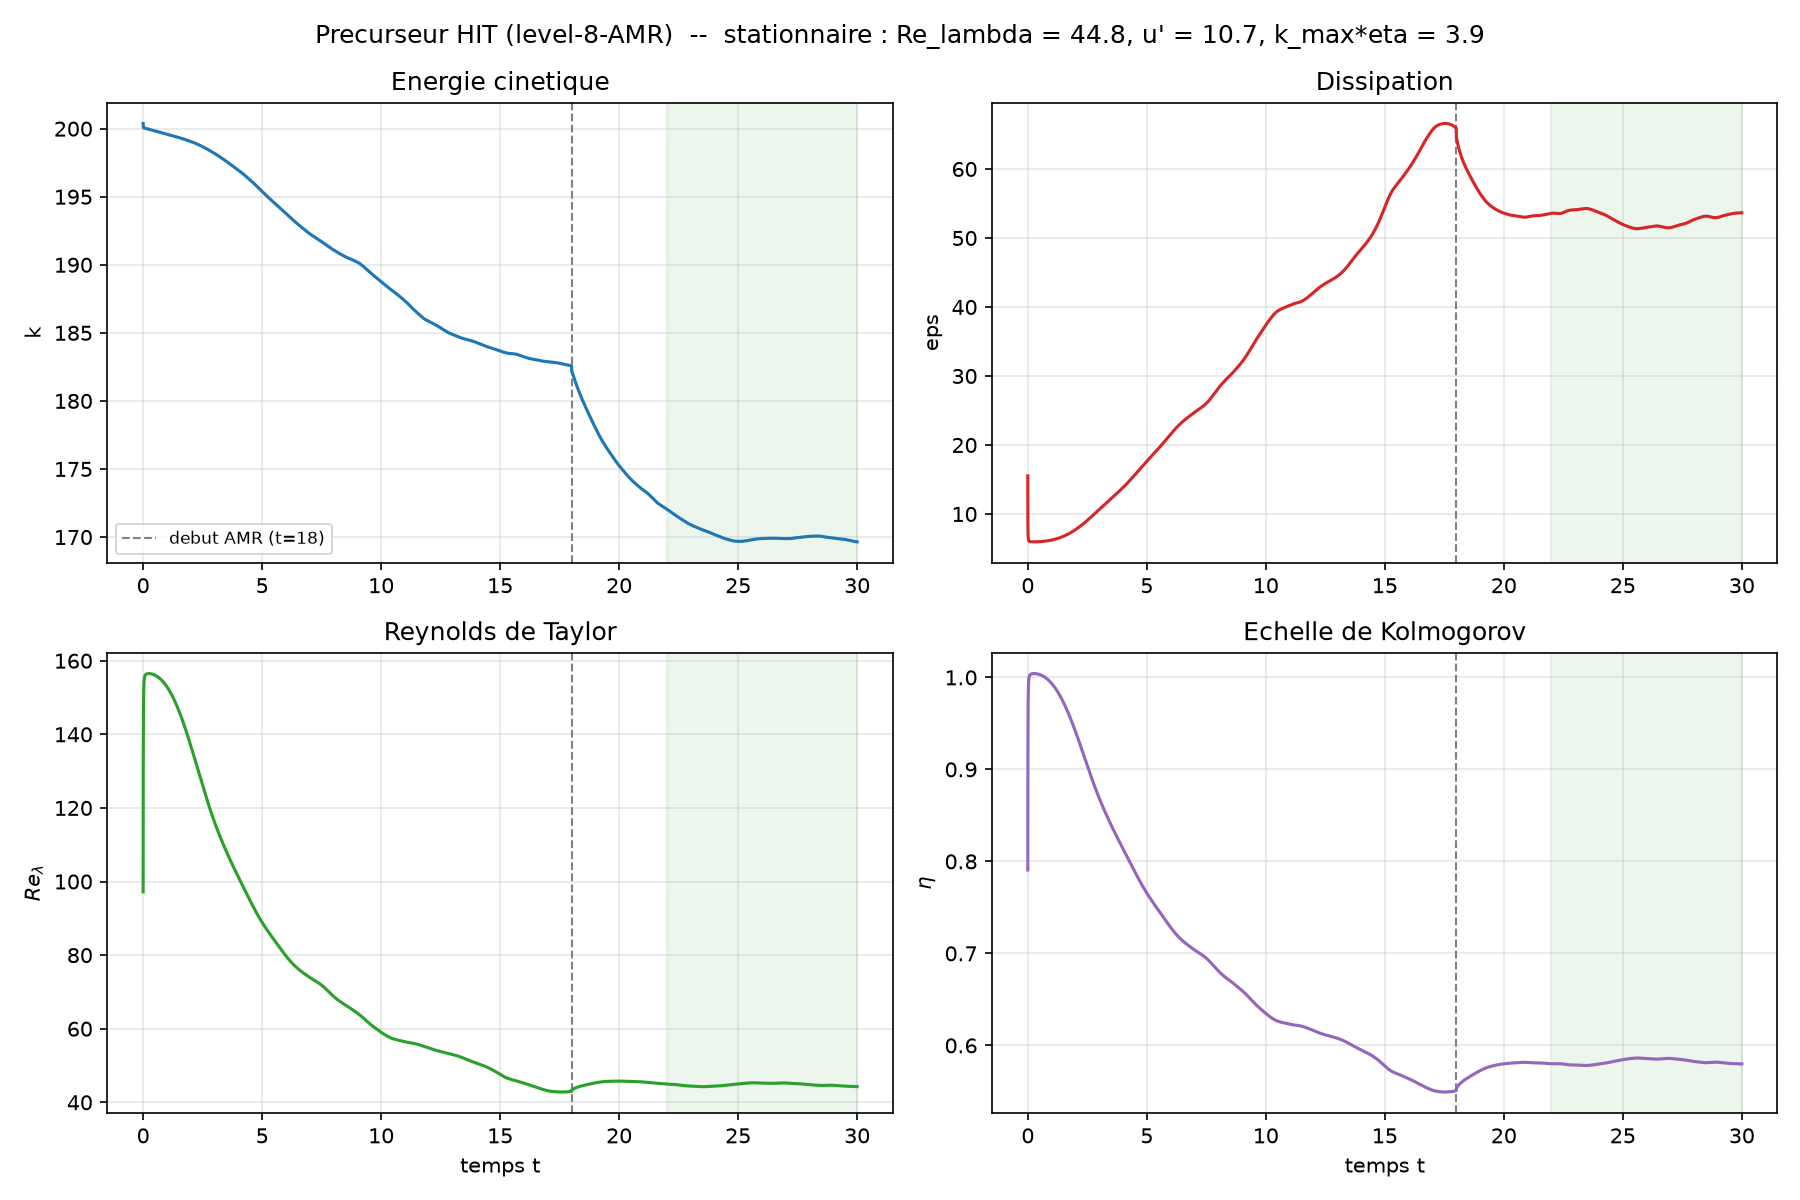
\includegraphics[width=\textwidth]{prec_carac.png}
    \end{column}
    \begin{column}{0.34\textwidth}
      \footnotesize
      \textbf{Lecture} :
      \begin{itemize}
        \item $\varepsilon$ part de la valeur d'un champ lisse,
              \textbf{croît} quand la cascade non linéaire s'installe
              (signature de la transition), culmine vers $t \approx 18$.
        \item $k$, $Re_\lambda$, $\eta$ atteignent un \textbf{plateau} :
              état statistiquement stationnaire pour $t \gtrsim 22$
              (bande verte = fenêtre de moyenne).
        \item Trait pointillé : bascule uniforme $\to$ AMR ($t=18$).
      \end{itemize}
      \vspace{0.3em}
      C'est \emph{dans cet état mûr} que la bulle est injectée
      (jamais dans un transitoire).
    \end{column}
  \end{columns}
\end{frame}

\begin{frame}{Caractérisation quantitative (moyennes sur $t \geq 22$)}
  \footnotesize
  \begin{columns}[T]
    \begin{column}{0.52\textwidth}
      \begin{tabular}{@{}llc@{}}
        \toprule
        \textbf{Grandeur} & \textbf{Symbole} & \textbf{Valeur} \\ \midrule
        Reynolds de Taylor      & $Re_\lambda$                        & $\mathbf{44{,}8}$ \\
        Reynolds intégral       & $Re_L = u'L/\nu$                    & $246$ \\
        Fluctuation rms         & $u' = \sqrt{2k/3}$                  & $10{,}65$ \\
        Énergie cinétique       & $k$                                 & $170{,}2$ \\
        Dissipation             & $\varepsilon$                       & $52{,}8$ \\ \midrule
        Échelle intégrale       & $L = k^{3/2}/\varepsilon$           & $42{,}1$ \\
        Micro-échelle de Taylor & $\lambda$                           & $7{,}67$ \\
        Échelle de Kolmogorov   & $\eta = (\nu^3/\varepsilon)^{1/4}$  & $0{,}582$ \\
        Temps de retournement   & $\tau_e = k/\varepsilon$            & $3{,}23$ \\
        \bottomrule
      \end{tabular}
      \vspace{0.3em}\\
      {\scriptsize Unités code : $\rho_1=1$, $g=1$, $L_0=120$, $D = 2R_0 = 16$.}
    \end{column}
    \begin{column}{0.48\textwidth}
      \begin{block}{Forçage linéaire contrôlé (Bassenne et al. 2016)}
        L'amplitude est ajustée à chaque pas pour que la puissance injectée
        compense la dissipation : $k$ est \textbf{tenue à une cible}
        \texttt{KE\_TARGET}. L'intensité turbulente devient un
        \emph{paramètre piloté} --- c'est la grandeur que l'étude fera varier.
      \end{block}
      \begin{itemize}
        \item Domaine périodique $\Rightarrow$ échelle intégrale
              $L \approx 42 \approx L_0/3$ : quelques grandes structures
              par côté, comportement attendu.
        \item IC = superposition de modes ABC $k=1,2,3$ + bruit (un mode
              seul = solution de Beltrami, ne transitionne \emph{jamais}).
      \end{itemize}
    \end{column}
  \end{columns}
\end{frame}

\begin{frame}{Toutes les échelles sont résolues --- aux trois niveaux}
  \footnotesize
  \textbf{Critère DNS standard (Pope)} : $k_{\max}\,\eta \gtrsim 1{,}5$, avec
  $k_{\max} = \pi\,2^{\text{lvl}}/L_0$ le plus grand nombre d'onde résolu.
  Champ $KE=200$ ($\eta = 0{,}582$) :
  \vspace{0.4em}
  \begin{center}
  \begin{tabular}{@{}lcccc@{}}
    \toprule
    & $\Delta x$ & $\bm{k_{\max}\,\eta}$ & $D/\Delta x$ (mailles/diam.) & couche limite $\delta/\Delta x$ \\
    \midrule
    \textbf{lvl 7} & $0{,}938$ & $1{,}95$ \textcolor{okgreen}{\checkmark} & $17$ \textcolor{warnred}{($<20$)} & $\approx 3$ \\
    \rowcolor{imftlight!15}
    \textbf{lvl 8} & $0{,}469$ & $\mathbf{3{,}90}$ \textcolor{okgreen}{\checkmark} & $34$ \textcolor{okgreen}{\checkmark} & $\approx 6$ \\
    \textbf{lvl 9} & $0{,}234$ & $7{,}80$ \textcolor{okgreen}{\checkmark} & $68$ \textcolor{okgreen}{\checkmark} & $\approx 12$ \\
    \bottomrule
  \end{tabular}
  \end{center}
  \vspace{0.4em}
  \begin{columns}[T]
    \begin{column}{0.55\textwidth}
      \begin{itemize}
        \item La gamme dissipative est capturée dès le niveau 7 ;
              au niveau 8, $\eta \approx 1{,}24\,\Delta x$ (sur-résolu).
        \item Couche limite de bulle : $Re_b = U_b D/\nu \approx 35$,
              $\delta \sim D/\sqrt{Re_b} \approx 2{,}7$ $\to$ $\approx 6$
              mailles au niveau 8 : cisaillement pariétal et sillage
              proche résolus.
      \end{itemize}
    \end{column}
    \begin{column}{0.45\textwidth}
      \begin{block}{Rôle de chaque niveau}
        \scriptsize
        lvl 7 = point grossier de la convergence ($17$ mailles/$D$, sous le
        seuil de $20$) ; lvl 8 = niveau de production pleinement résolu ;
        lvl 9 = vérification (différé : nécessite de plafonner l'AMR
        vorticité au niveau 8).
      \end{block}
    \end{column}
  \end{columns}
\end{frame}

%==============================================================================
\section{Visualisation des structures turbulentes}
%==============================================================================
\begin{frame}{Maillage adaptatif et structures 3D}
  \begin{columns}[c]
    \begin{column}{0.5\textwidth}
      \centering
      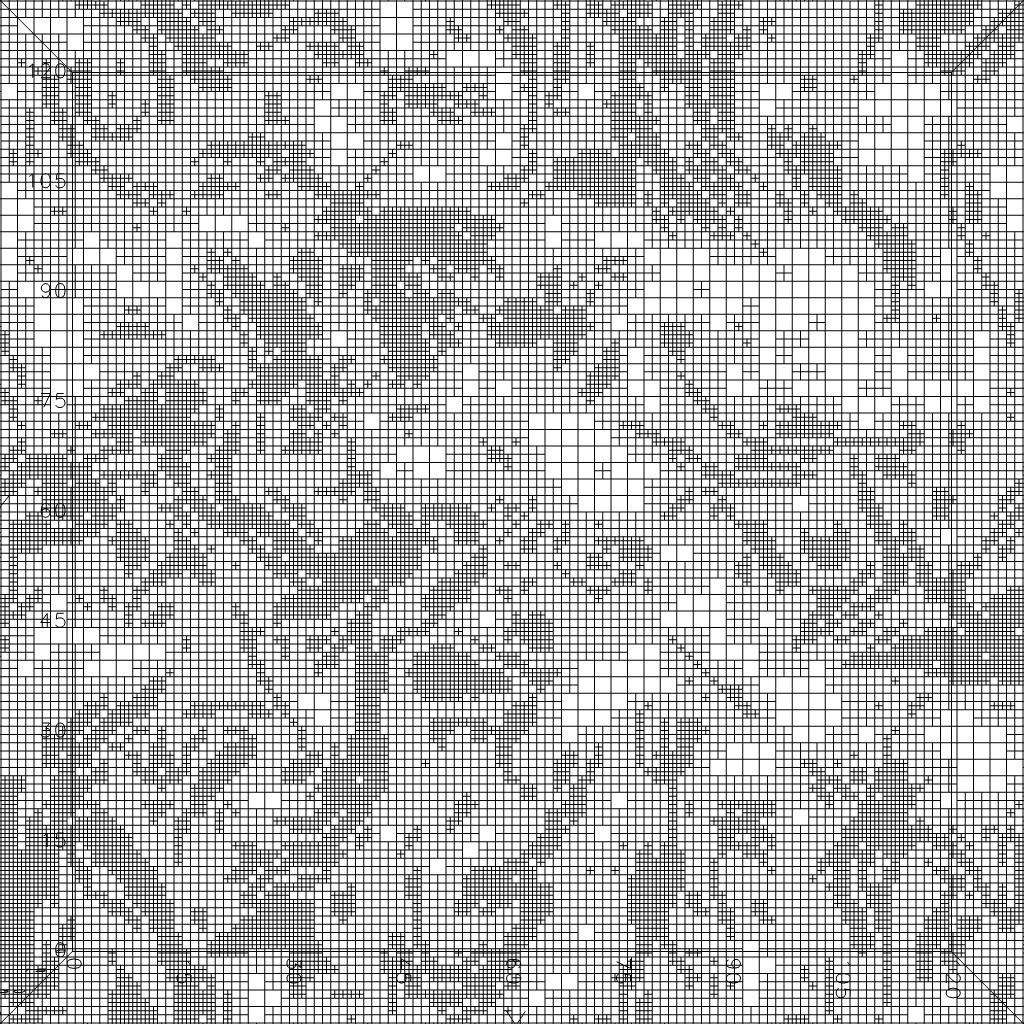
\includegraphics[width=0.92\textwidth,height=0.58\textheight,keepaspectratio]{prec_maillage.png}\\
      {\scriptsize Maillage adaptatif (coupe $z$ à mi-domaine) : les mailles
       fines suivent les filaments de vorticité, les zones lisses
       grossissent.}
    \end{column}
    \begin{column}{0.5\textwidth}
      \centering
      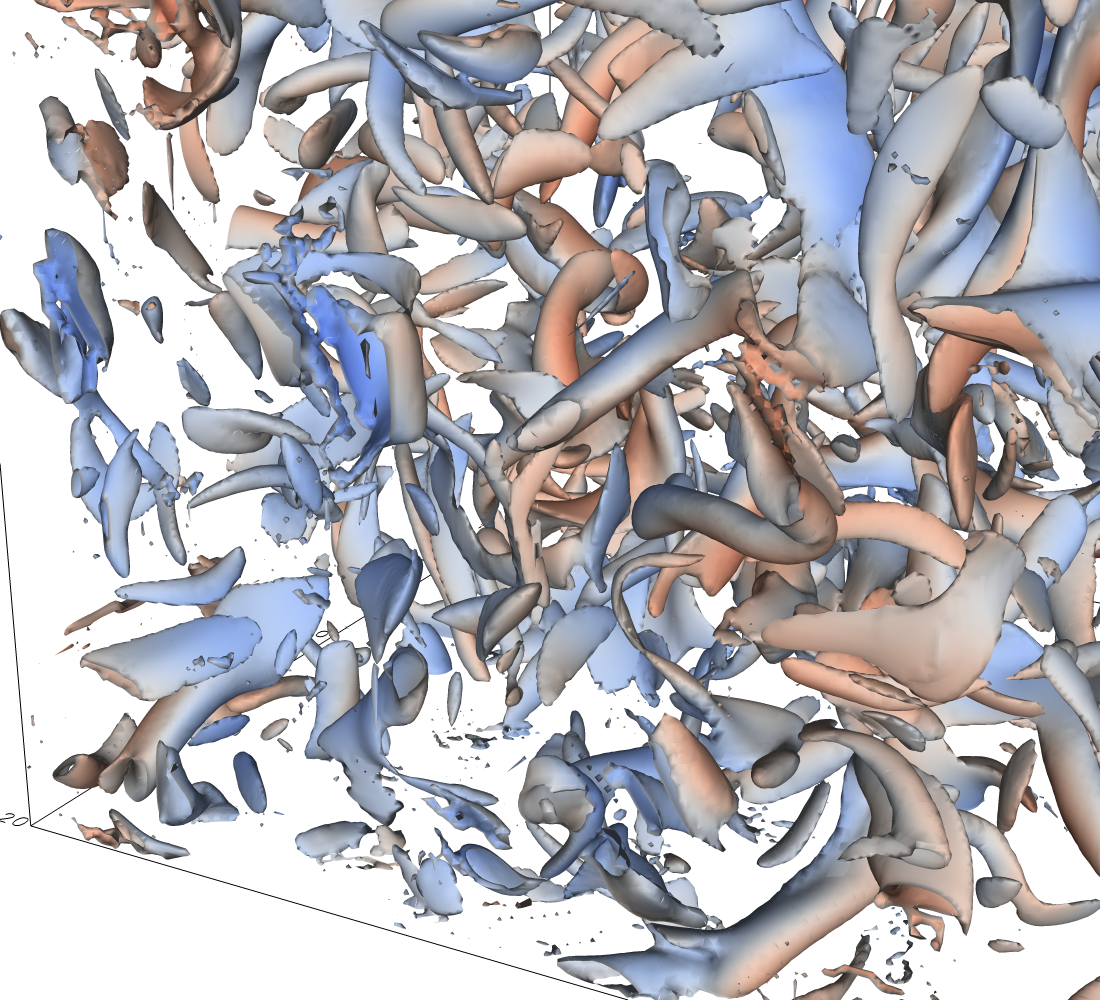
\includegraphics[width=0.92\textwidth,height=0.58\textheight,keepaspectratio]{prec_vortex3d.png}\\
      {\scriptsize Isosurface 3D de $|\boldsymbol\omega|$ (seuil
       $1{,}5\,\omega_{rms}$), colorée par $u_z$ : tubes tourbillonnaires
       en \og vermicelles \fg{}, signature classique de la THI.}
    \end{column}
  \end{columns}
\end{frame}

\begin{frame}{Champs sur une coupe à mi-domaine ($t=25$, champ mûr)}
  \begin{columns}[c]
    \begin{column}{0.33\textwidth}
      \centering
      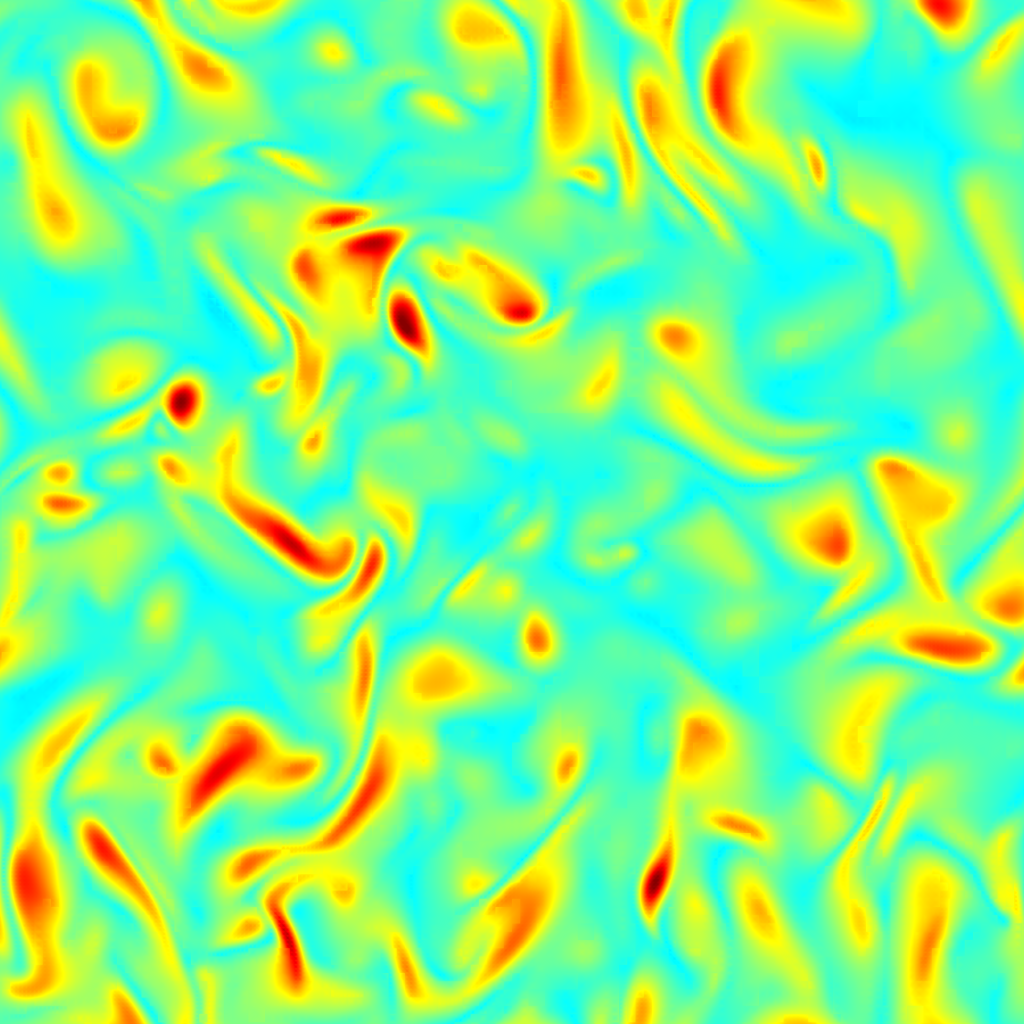
\includegraphics[width=\textwidth]{prec_vorticite.png}\\
      {\scriptsize Vorticité $|\boldsymbol\omega|$}
    \end{column}
    \begin{column}{0.33\textwidth}
      \centering
      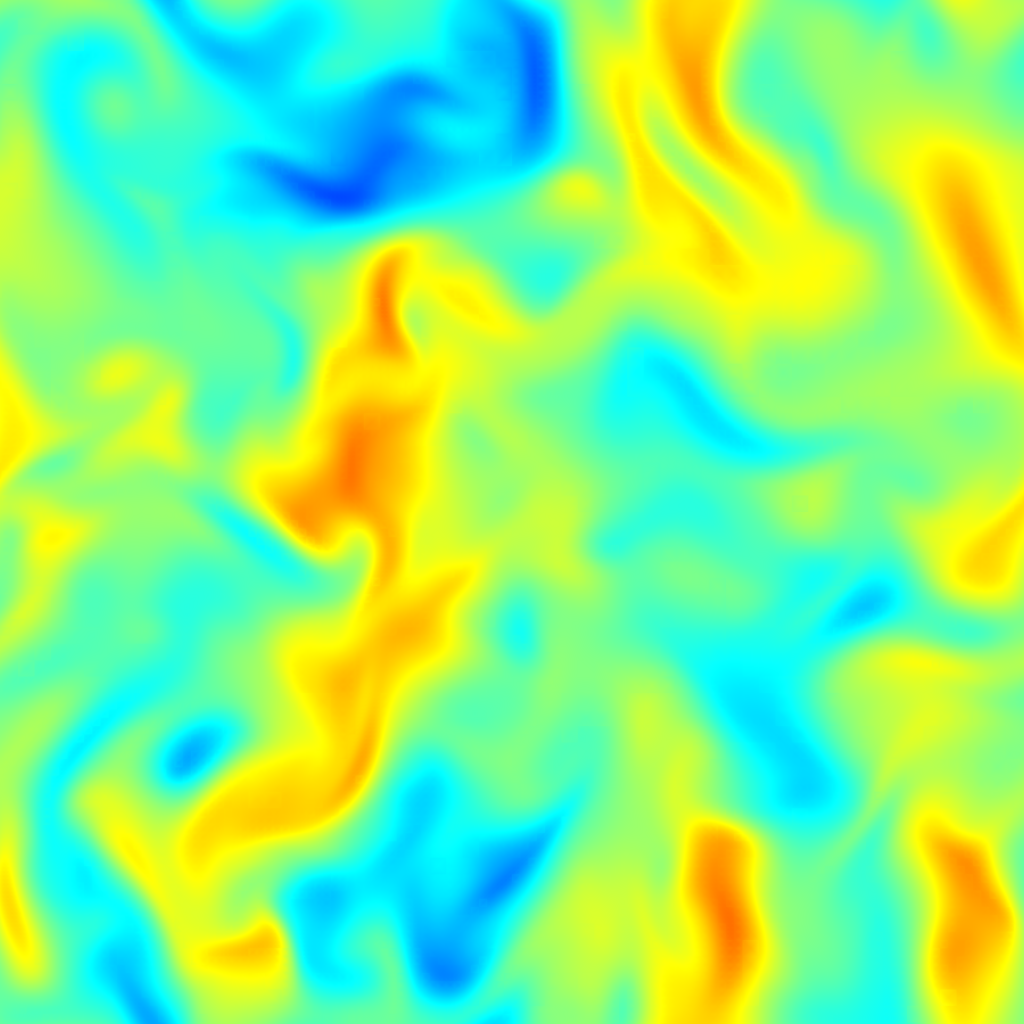
\includegraphics[width=\textwidth]{prec_vitesse.png}\\
      {\scriptsize Vitesse verticale $u_z$}
    \end{column}
    \begin{column}{0.33\textwidth}
      \centering
      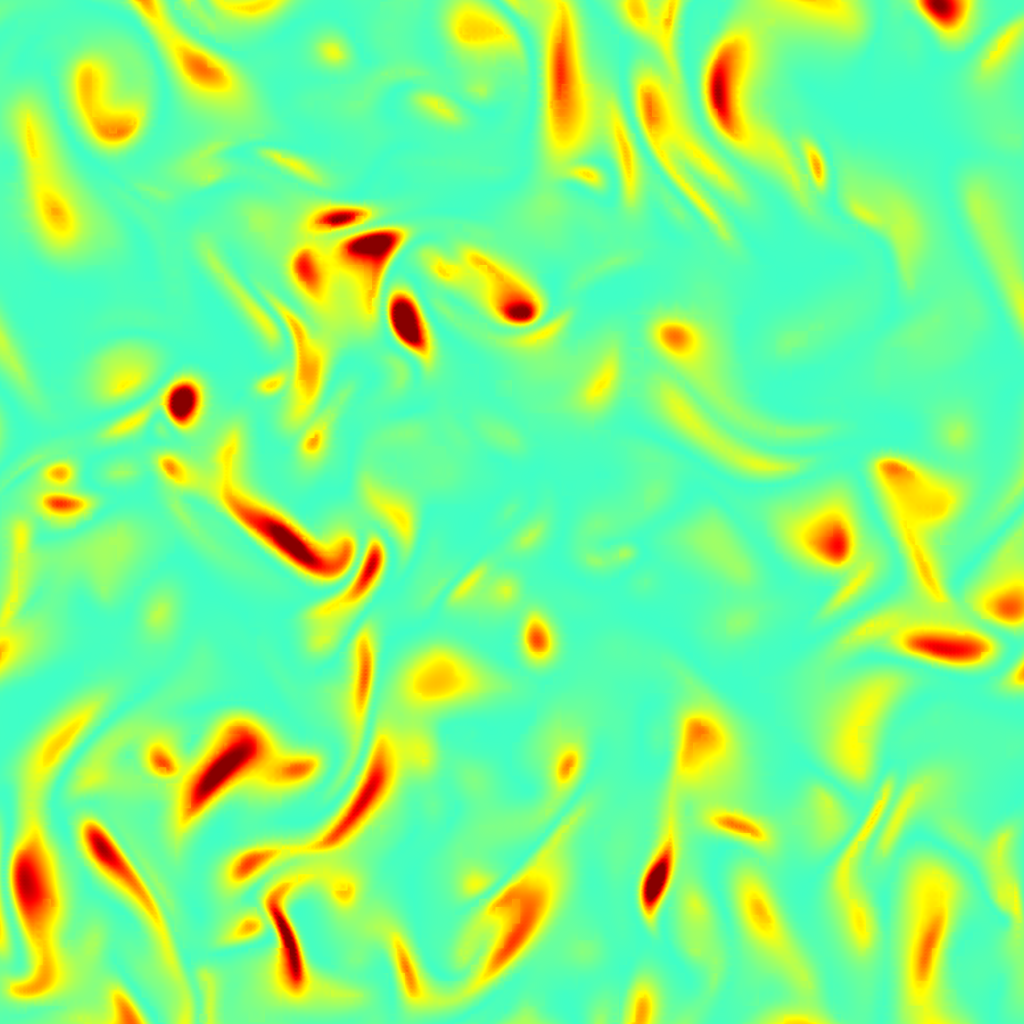
\includegraphics[width=\textwidth]{prec_enstrophie.png}\\
      {\scriptsize Enstrophie $|\boldsymbol\omega|^2$}
    \end{column}
  \end{columns}
  \vspace{0.5em}
  \begin{center}
    \footnotesize
    Structures lisses et continues $\Rightarrow$ bien résolues (pas de bruit
    maille-à-maille). Des \textbf{films} de l'évolution temporelle
    ($t \in [19,30]$ : vitesse, vorticité, isosurface 3D) ont aussi été
    produits (\texttt{scripts/figures/films/}).
  \end{center}
\end{frame}

%==============================================================================
\section{Bulle à $We_t \approx 11$ : fragmentation}
%==============================================================================
\begin{frame}{Premier run bulle complet (lvl 7) : la bulle ne survit pas}
  \footnotesize
  Bulle injectée dans le champ précédent à $t=30$, suivie $50$ unités de temps.
  Solveur numériquement sain (mailles, pas de temps, multigrille : rien à
  signaler). Volume à l'injection : $94\,\%$ du théorique. \textbf{Mais :}
  \vspace{0.4em}
  \begin{center}
  \begin{tabular}{@{}lp{9.2cm}@{}}
    \toprule
    \textbf{Instant} & \textbf{Observation} \\
    \midrule
    $t=30$ (injection) & Volume $=2021$ ($94\,\%$) ; $d_{eq} = 15{,}7 \approx 2R_0$. \\
    $t=34$ & Étirement extrême : boîte englobante à $44$ sur un axe
             ($\approx 3\times$ le diamètre) --- ligament avant pincement. \\
    \rowcolor{warnred!12}
    $t \approx 38$--$41$ & \textbf{Rupture} : volume de la région mère
             $1335 \to 250$ ($-88\,\%$) ; $d_{eq}$ final $= 7{,}3$. \\
    $t=46$ & Pic de déformation $\chi = 4{,}60$ (fragment en cours de déchirement). \\
    $t \to 80$ & Sauts de volume $\pm 20$--$39\,\%$ en un pas : le tag
             \og mère \fg{} bascule entre fragments comparables. \\
    \bottomrule
  \end{tabular}
  \end{center}
  \vspace{0.3em}
  \begin{center}
    \textcolor{warnred}{\textbf{Cohérent avec le régime annoncé par la
    caractérisation : $We_t \approx 11 \gg 1$.}}
  \end{center}
\end{frame}

\begin{frame}{La rupture en images : la turbulence gagne, malgré $Bo = 1$}
  \begin{columns}[c]
    \begin{column}{0.19\textwidth}
      \centering
      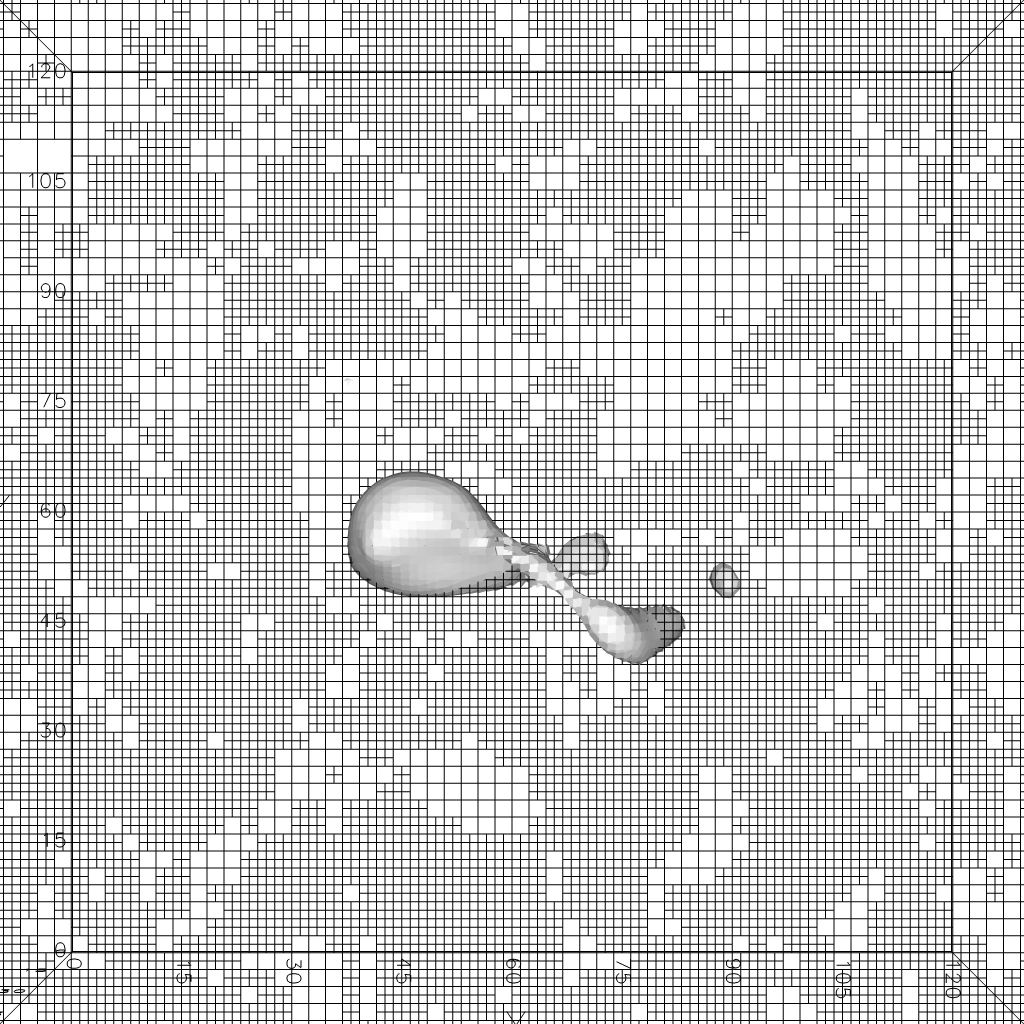
\includegraphics[width=\textwidth]{bulle_lvl7_t31.png}\\
      {\scriptsize $t=31$ : intacte mais très déformée}
    \end{column}
    \begin{column}{0.19\textwidth}
      \centering
      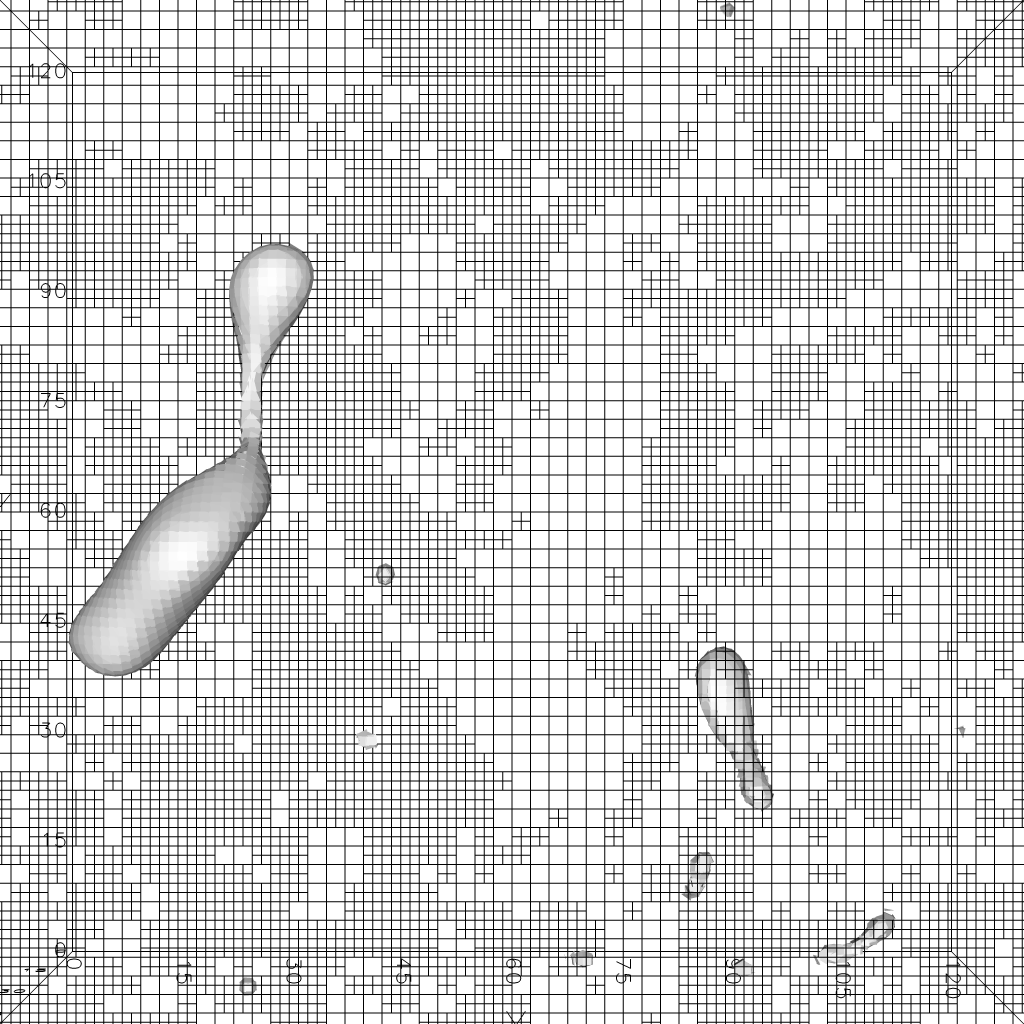
\includegraphics[width=\textwidth]{bulle_lvl7_t34.png}\\
      {\scriptsize $t=34$ : intacte mais très déformée}
    \end{column}
    \begin{column}{0.19\textwidth}
      \centering
      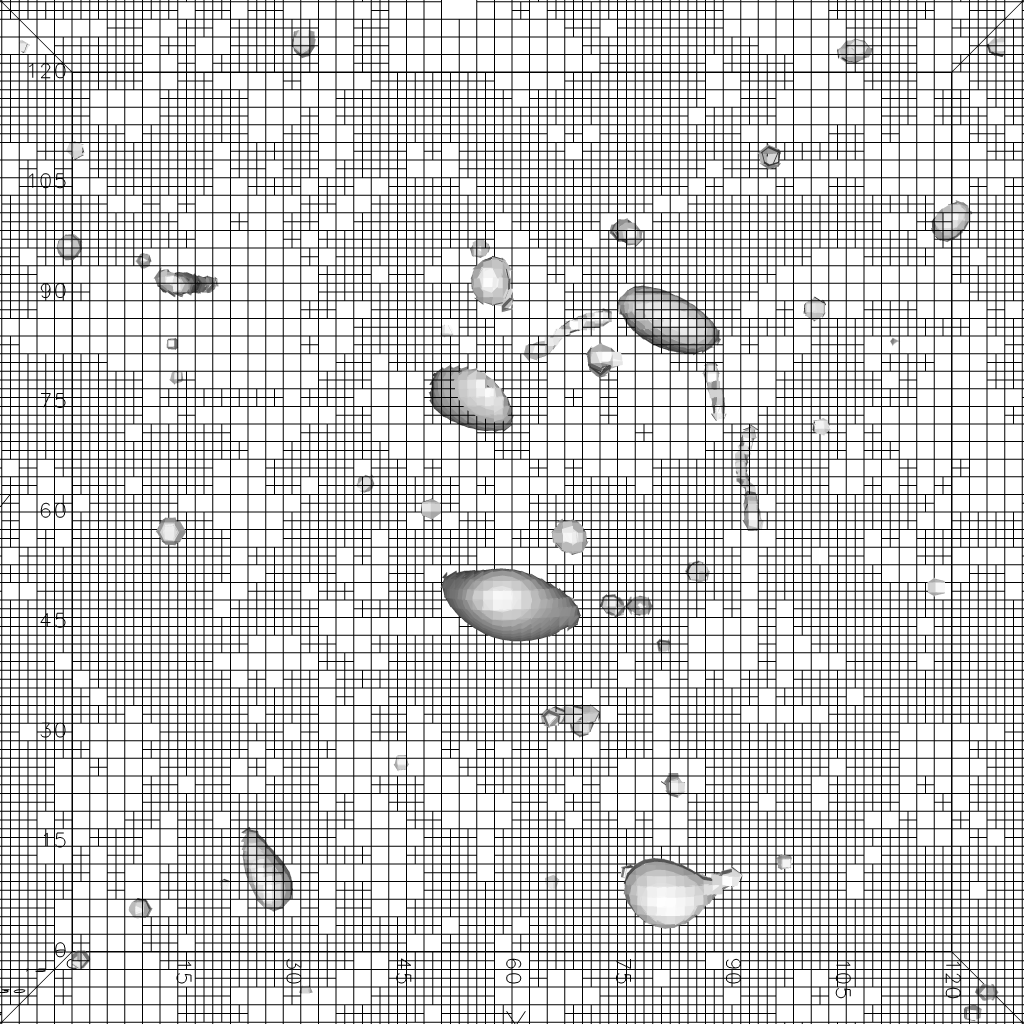
\includegraphics[width=\textwidth]{bulle_lvl7_t39.png}\\
      {\scriptsize $t=39$ : \textcolor{warnred}{rupture}}
    \end{column}
    \begin{column}{0.19\textwidth}
      \centering
      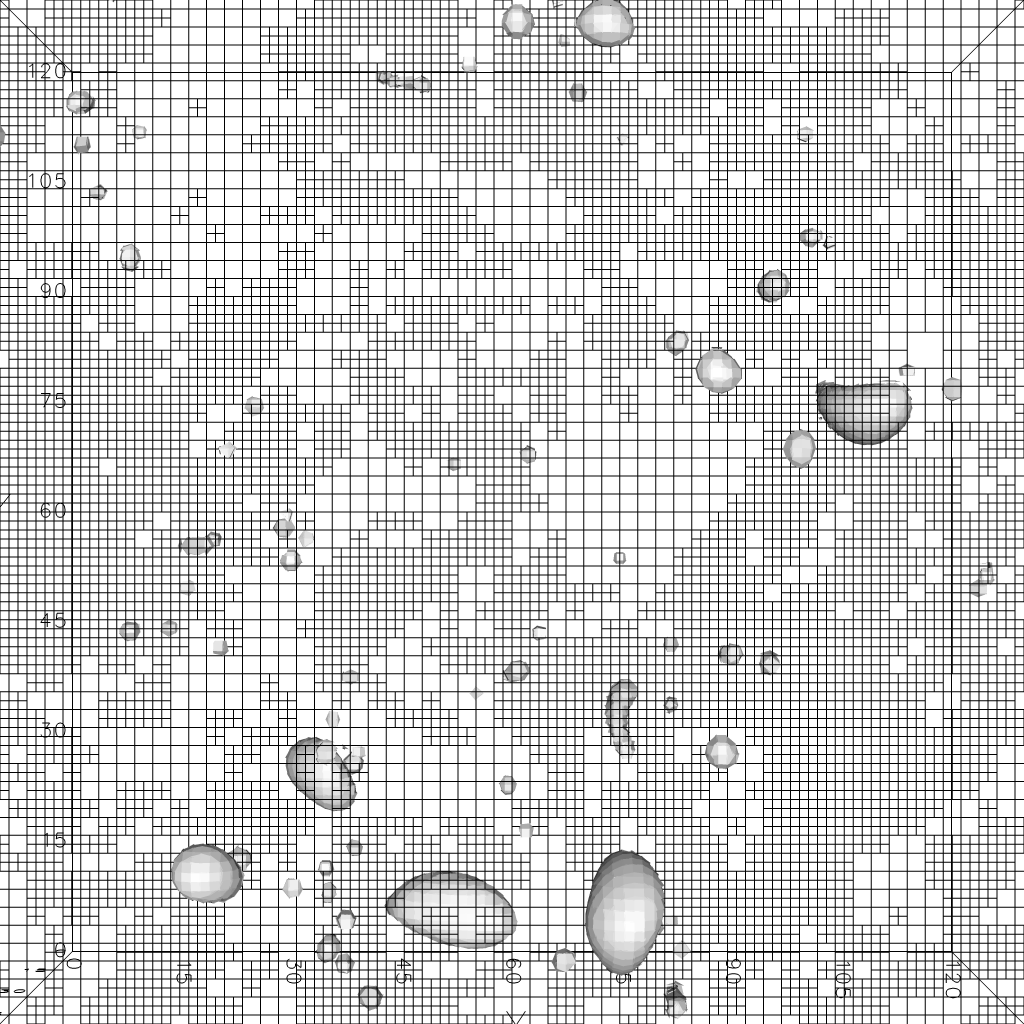
\includegraphics[width=\textwidth]{bulle_lvl7_t42.png}\\
      {\scriptsize $t=42$ : fragments}
    \end{column}
    \begin{column}{0.19\textwidth}
      \centering
      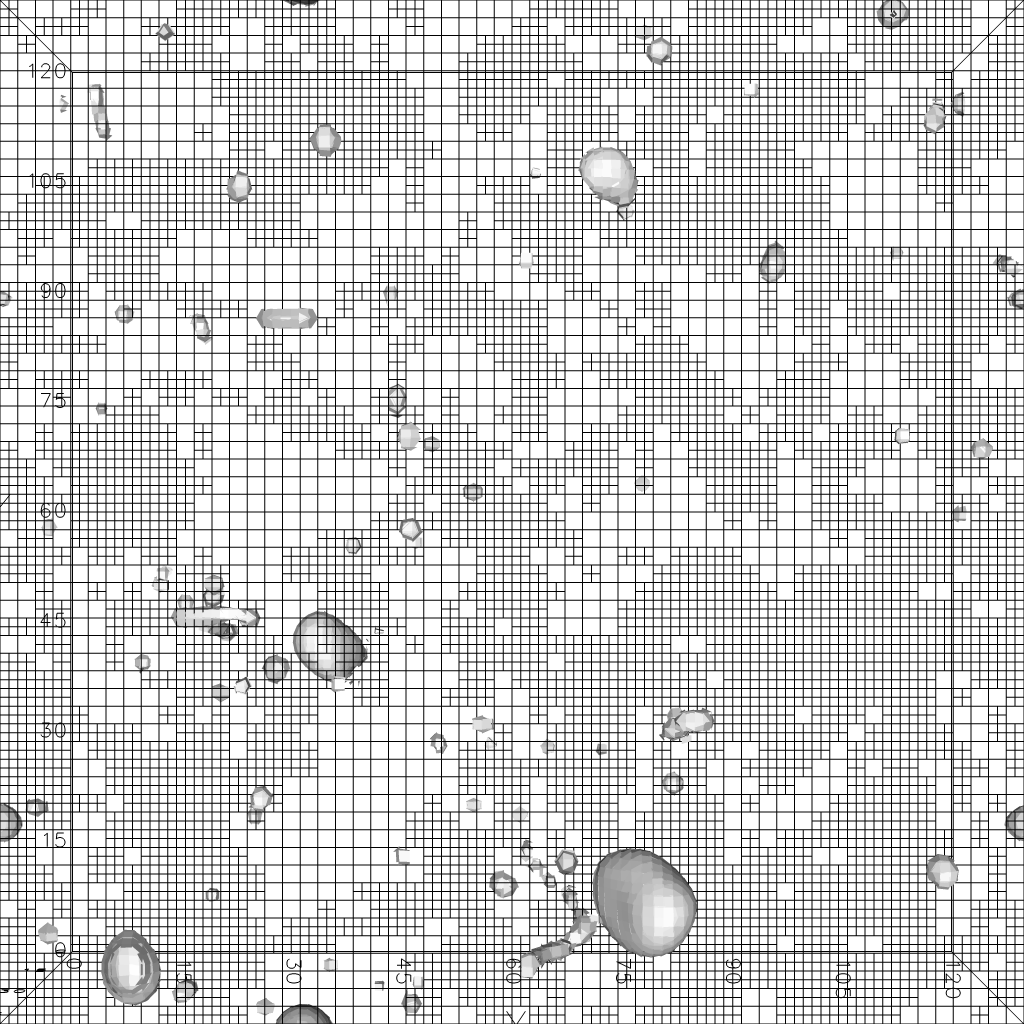
\includegraphics[width=\textwidth]{bulle_lvl7_t46.png}\\
      {\scriptsize $t=46$ : non exploitable}
    \end{column}
  \end{columns}
  \vspace{0.5em}
  \begin{columns}[T]
    \begin{column}{0.55\textwidth}
      \footnotesize
      À $Bo = 1$, la tension de surface \emph{équilibre} la flottabilité :
      seule en ascension, cette bulle resterait entière (régime
      ellipsoïdal). C'est bien la \textbf{turbulence} ($We_t \approx 11$)
      qui la déchire : étirement en ligament par les tourbillons, pincement,
      puis cascade de fragmentations.
    \end{column}
    \begin{column}{0.45\textwidth}
      \begin{block}{Film disponible}
        \footnotesize
        Animation complète (interface + maillage, $t = 31 \to 80$) :
        \texttt{films/bulle\_lvl7\_we11\_rupture.mp4} --- à projeter
        pendant la présentation.
      \end{block}
    \end{column}
  \end{columns}
\end{frame}

\begin{frame}{Signaux de la rupture : vitesse et déformation}
  \begin{columns}[c]
    \begin{column}{0.46\textwidth}
      \centering
      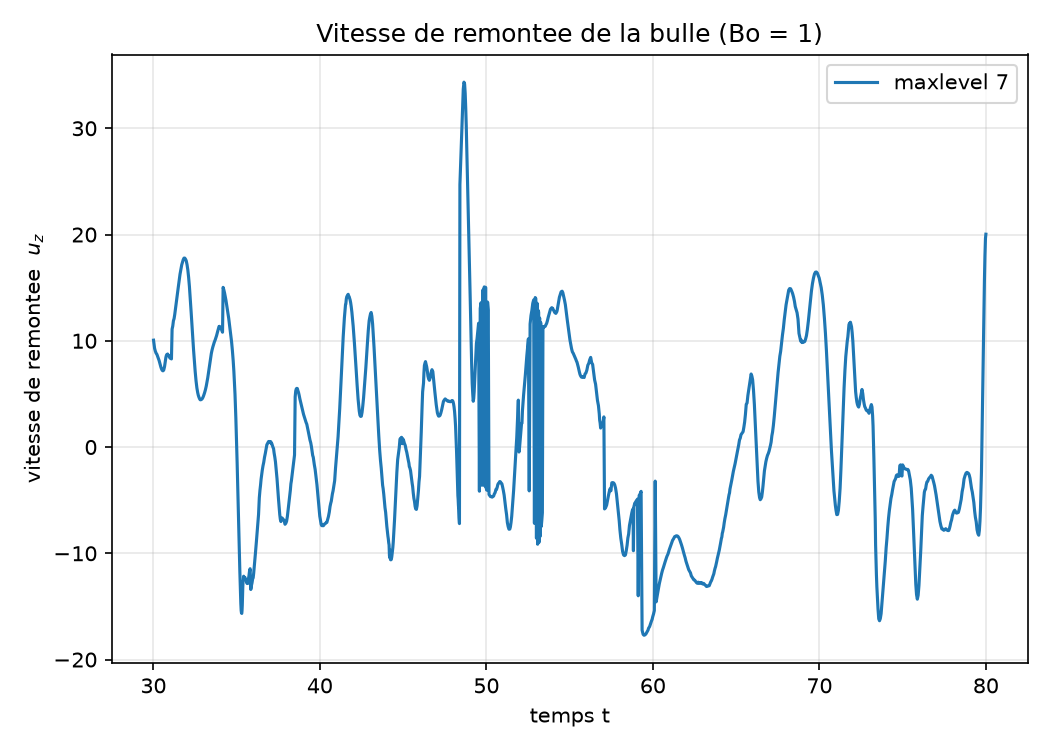
\includegraphics[width=\textwidth]{bulle_lvl7_uz.png}\\
      {\scriptsize $u_z(t)$ de la région mère : aucun plateau, oscillations
       $-17{,}7$ à $+34{,}3$ (écart-type $9{,}2$). Pas de vitesse terminale
       définissable.}
    \end{column}
    \begin{column}{0.54\textwidth}
      \centering
      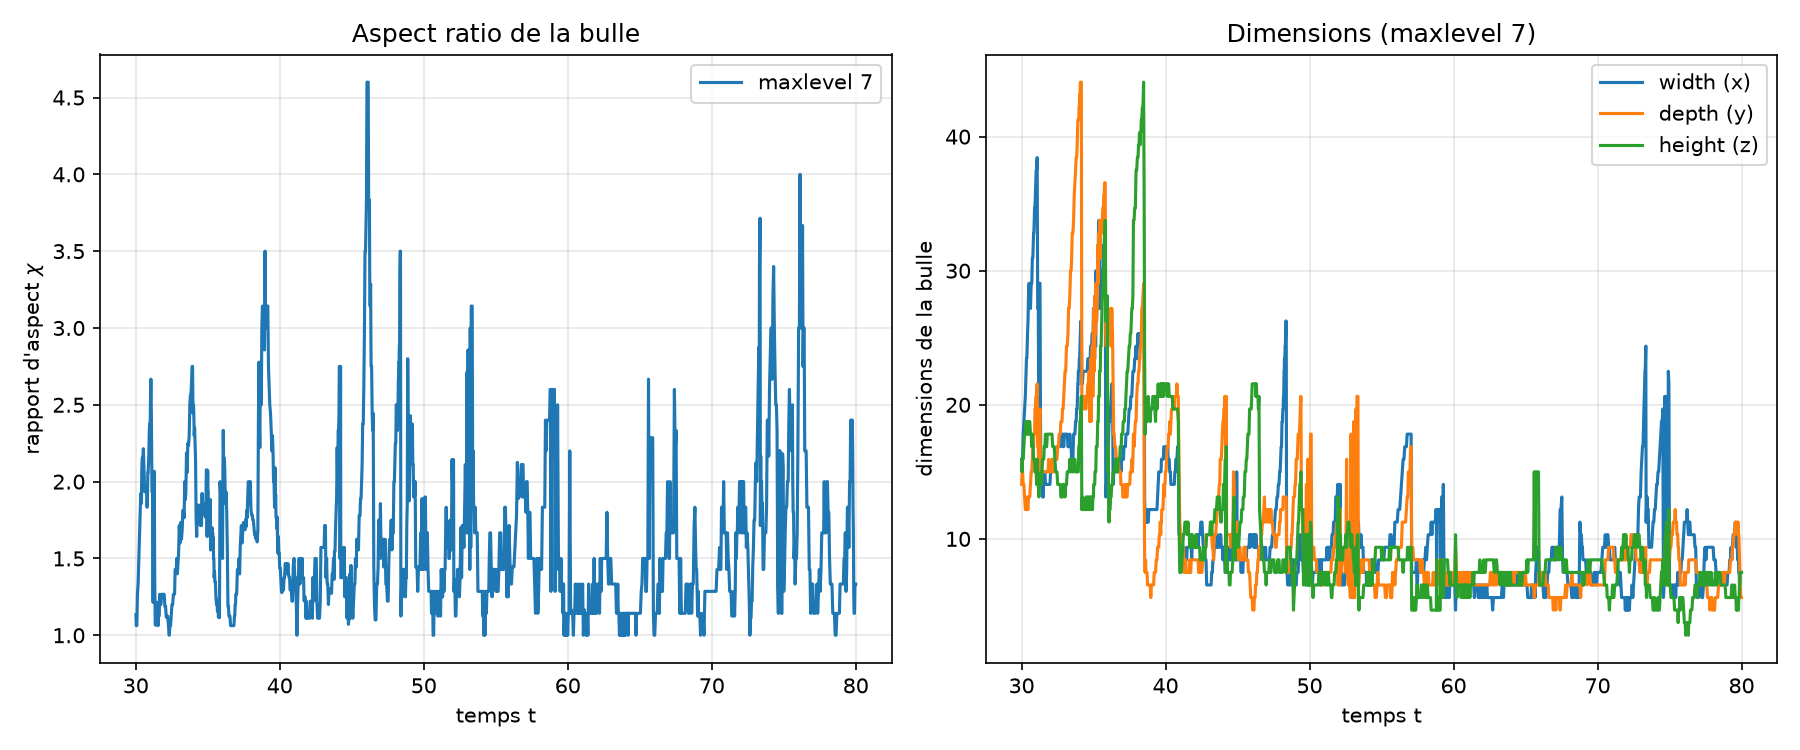
\includegraphics[width=\textwidth]{bulle_lvl7_aspect.png}\\
      {\scriptsize $\chi(t)$ et dimensions de la boîte englobante : la chute
       des trois dimensions après $t \approx 40$ ($44 \to 5$--$10$) marque
       la rupture.}
    \end{column}
  \end{columns}
\end{frame}

\begin{frame}{Trajectoire, et la limite du suivi \og bulle mère \fg{}}
  \begin{columns}[c]
    \begin{column}{0.58\textwidth}
      \centering
      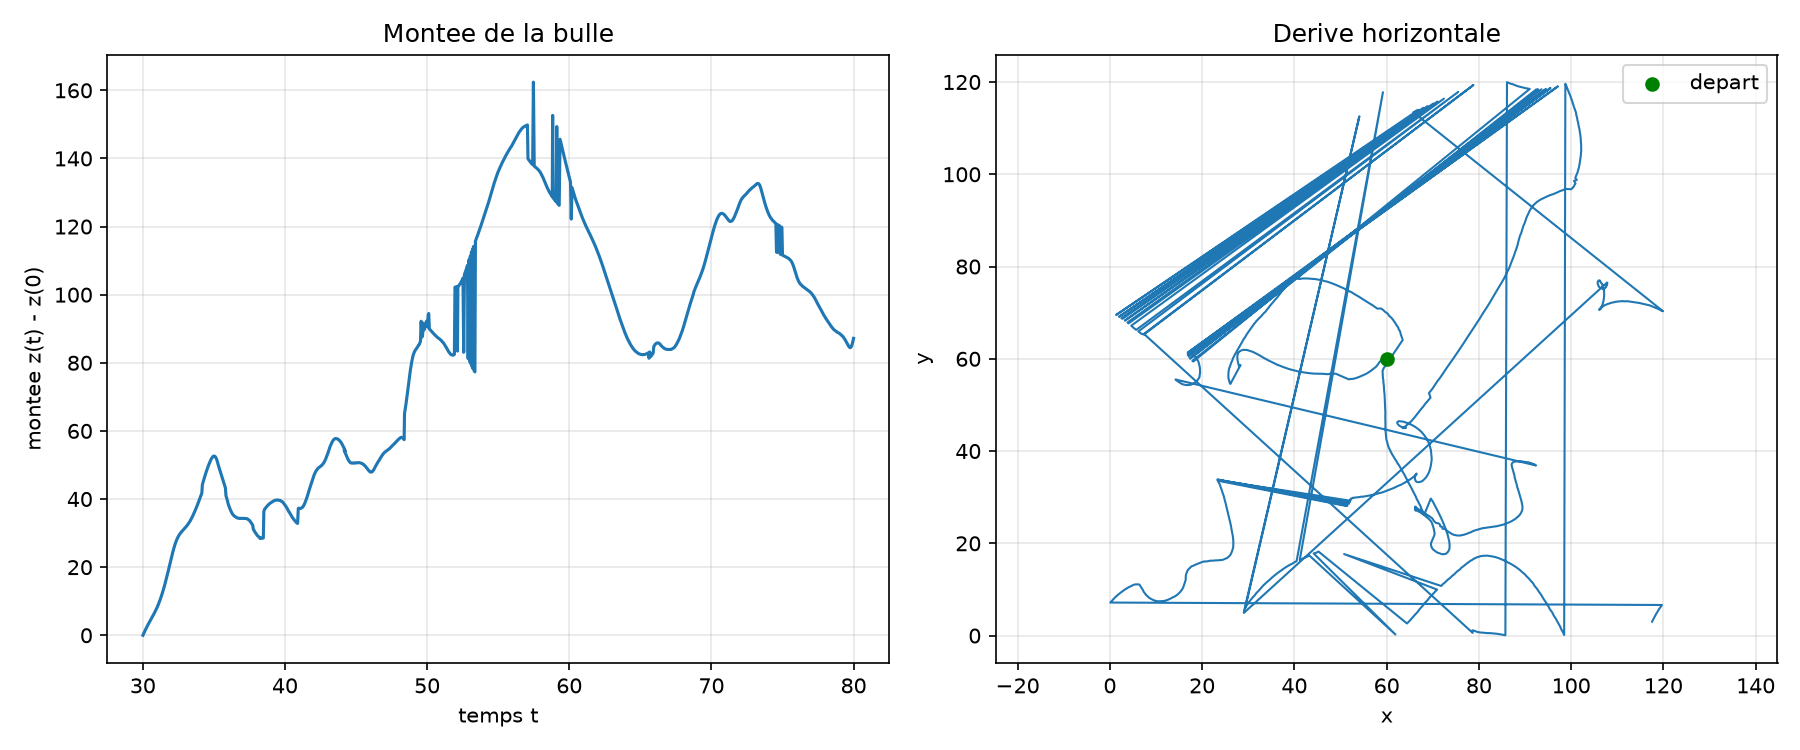
\includegraphics[width=\textwidth]{bulle_lvl7_trajectoire.png}\\
      {\scriptsize Montée $z(t)$ (gauche) et dérive horizontale (droite).
       Les segments rectilignes traversant le domaine = changements
       d'identité de fragment, pas une dérive physique.}
    \end{column}
    \begin{column}{0.42\textwidth}
      \begin{alertblock}{Limite méthodologique}
        \footnotesize
        Le code suit la plus grande région gazeuse (\texttt{tag}), en
        supposant \og $Bo=1$ : pas de fragmentation \fg{}. Faux à
        $We_t \approx 11$ : après rupture, la \og vitesse terminale \fg{}
        moyennée ($-1{,}95$) ne décrit qu'\emph{un fragment parmi d'autres}
        --- inutilisable pour la traînée.
      \end{alertblock}
      \footnotesize
      Le point lvl7-$We_t{=}11$ reste \emph{utile} : c'est une observation
      du \textbf{seuil de rupture turbulente} pour l'étude
      intensité $\to$ vitesse, mais pas un point de convergence de maillage.
    \end{column}
  \end{columns}
\end{frame}

\begin{frame}{Verdict : ce n'est pas $Bo$, c'est $We_t$}
  \begin{columns}[T]
    \begin{column}{0.5\textwidth}
      \begin{block}{Vérification : $Bo = 1$ est bien tenu}
        \footnotesize
        La tension de surface est imposée \emph{dynamiquement} dans le code :
        $\sigma = (\rho_1{-}\rho_2)\,|g|\,(2R_0)^2 = 255{,}7$
        $\Rightarrow Bo = \Delta\rho\,g\,D^2/\sigma = \mathbf{1{,}000}$
        exactement (vérifié). La rupture n'est \textbf{pas} un problème
        de Bond.
      \end{block}
      \textbf{Le vrai coupable} :
      \[ We_t = \frac{2\rho_\ell\,(\varepsilon D)^{2/3}\,D}{\sigma}
         = \mathbf{11{,}2} \quad (KE{=}200) \]
      contraintes turbulentes $\gg$ tension de surface : la bulle est
      déchirée en $\sim 9$ unités de temps, malgré $Bo=1$.
      À cette intensité, $I = u'/U_b = 2{,}66$ : les fluctuations dominent
      complètement la flottabilité.
    \end{column}
    \begin{column}{0.5\textwidth}
      \begin{block}{Ce que dit la littérature}
        \footnotesize
        Le Weber \textbf{critique} de rupture d'une bulle en turbulence est
        de l'ordre de l'\textbf{unité} : $We_c \sim 1$--$3$ selon les
        études (Hinze 1955 ; Risso \& Fabre, JFM 1998 ; Rivière et al.,
        JFM 2021 ; Perrard et al., JFM 2021). En dessous, la bulle se
        \emph{déforme} sous les tourbillons mais \textbf{ne casse pas}.
      \end{block}
      \begin{block}{Décision (appuyée par cette biblio)}
        Viser $\bm{We_t \approx 1}$ : à la frontière du régime de rupture
        --- déformation maximale \emph{sans} fragmentation, condition
        nécessaire pour mesurer vitesse terminale et traînée.
      \end{block}
      \footnotesize
      Bonus : turbulence plus douce $\Rightarrow$ $\eta$ plus grand
      $\Rightarrow$ maillage moins chargé $\Rightarrow$ solveur diphasique
      niveau 8 nettement plus rapide.
    \end{column}
  \end{columns}
\end{frame}

%==============================================================================
\section{Ré-équilibrage vers $We_t \approx 1$}
%==============================================================================
\begin{frame}{Le nouveau champ : $We_t = 0{,}97$ --- cible atteinte}
  \footnotesize
  \begin{columns}[T]
    \begin{column}{0.56\textwidth}
      \begin{tabular}{@{}lcc@{}}
        \toprule
        \textbf{Grandeur} & \textbf{$KE{=}200$} & \textbf{$KE{=}15$} \\
        \midrule
        Énergie cinétique $k$        & $170{,}2$  & $14{,}97$ \\
        Dissipation $\varepsilon$    & $52{,}8$   & $1{,}35$ \\
        Fluctuation rms $u'$         & $10{,}65$  & $3{,}16$ \\
        $Re_\lambda$                 & $44{,}8$   & $24{,}6$ \\
        Échelle de Kolmogorov $\eta$ & $0{,}582$  & $1{,}456$ \\
        $k_{\max}\,\eta$ (lvl 8)     & $3{,}90$   & $\mathbf{9{,}76}$ \\
        $k_{\max}\,\eta$ (lvl 7)     & $1{,}95$   & $4{,}88$ \\
        Intensité $I = u'/U_b$       & $2{,}66$   & $0{,}79$ \\
        \rowcolor{okgreen!15}
        \textbf{Weber turbulent} $We_t$ & $\approx 11$ & $\mathbf{0{,}97}$ \\
        \bottomrule
      \end{tabular}
    \end{column}
    \begin{column}{0.44\textwidth}
      \begin{itemize}
        \item $We_t = 0{,}97$ : la cible $\approx 1$ est atteinte
              quasi exactement.
        \item La résolution s'\emph{améliore} : turbulence plus douce
              $\Rightarrow$ $\eta$ plus grand $\Rightarrow$
              $k_{\max}\eta = 9{,}8$ au niveau 8, et même le niveau 7
              est très largement au-dessus du critère.
        \item $I = 0{,}79$ : flottabilité et fluctuations du même ordre
              --- le régime intéressant pour la question
              \og la turbulence accélère-t-elle ou freine-t-elle
              la remontée ? \fg{}
        \item Maillage bien moins chargé ($\approx 1{,}3$~M mailles pour le
              champ $KE=15$, contre $6{,}6$~M à $KE=200$) $\Rightarrow$ runs
              relancés avec \emph{moins} de cœurs (8 et 32 au lieu de 32 et 64).
      \end{itemize}
    \end{column}
  \end{columns}
\end{frame}

\begin{frame}{Le champ $We_t \approx 1$ en images}
  \begin{columns}[c]
    \begin{column}{0.25\textwidth}
      \centering
      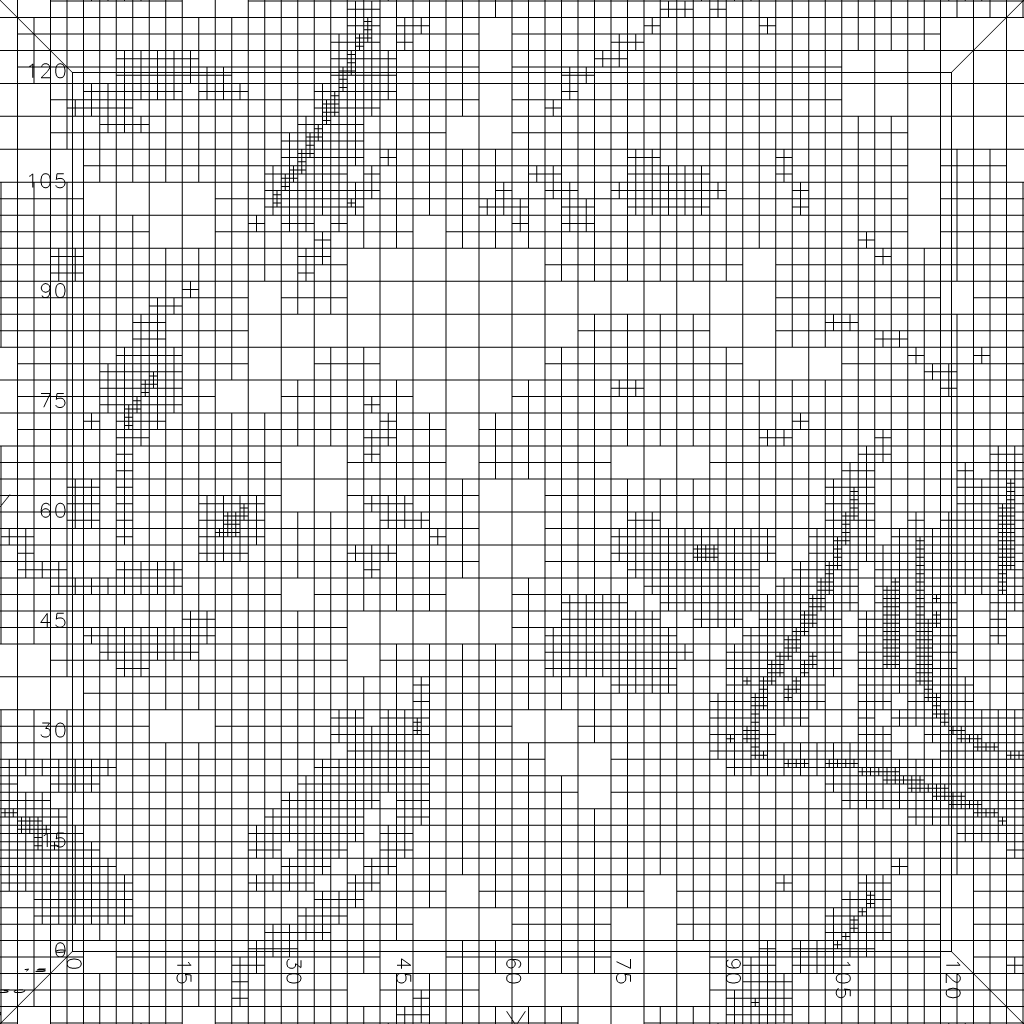
\includegraphics[width=\textwidth,height=0.34\textheight,keepaspectratio]{prec_maillage_we1.png}\\
      {\scriptsize Maillage adaptatif}
    \end{column}
    \begin{column}{0.25\textwidth}
      \centering
      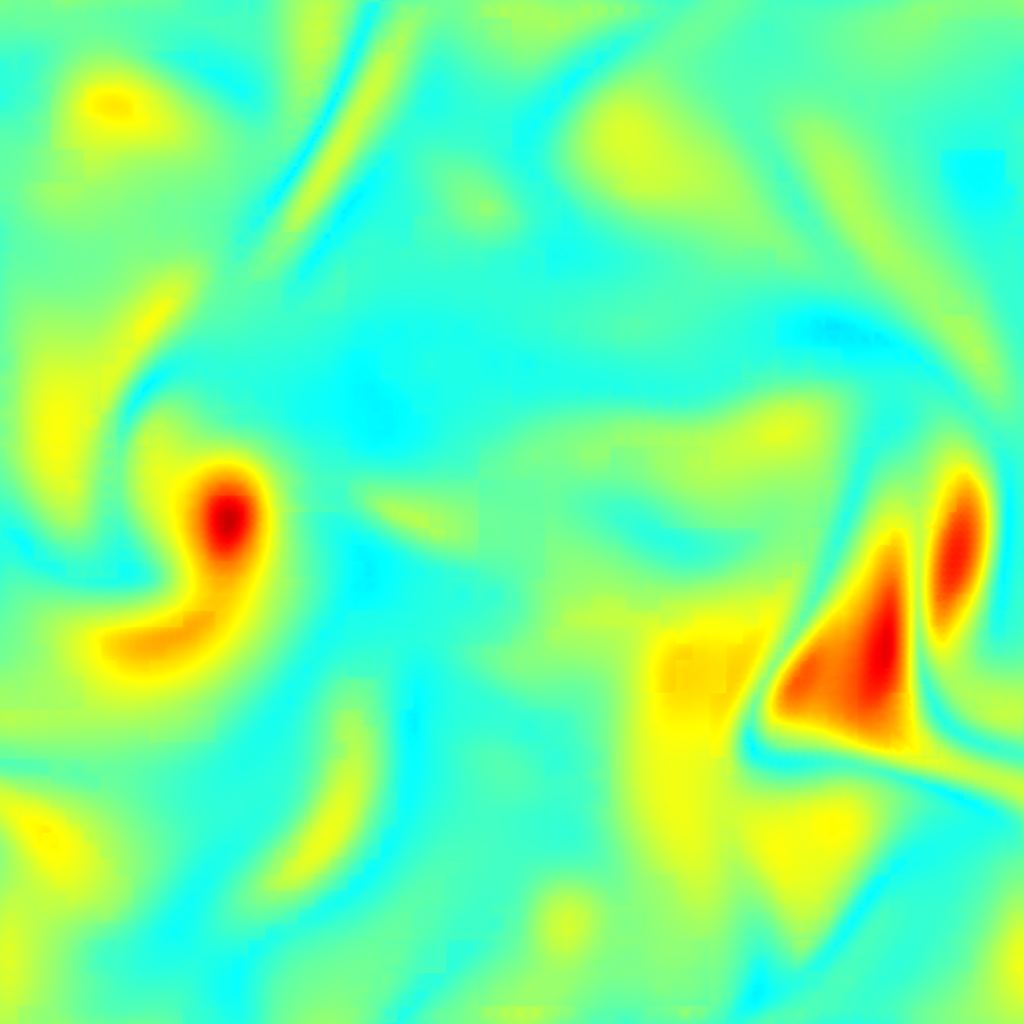
\includegraphics[width=\textwidth,height=0.34\textheight,keepaspectratio]{prec_vorticite_we1.png}\\
      {\scriptsize Vorticité $|\boldsymbol\omega|$}
    \end{column}
    \begin{column}{0.25\textwidth}
      \centering
      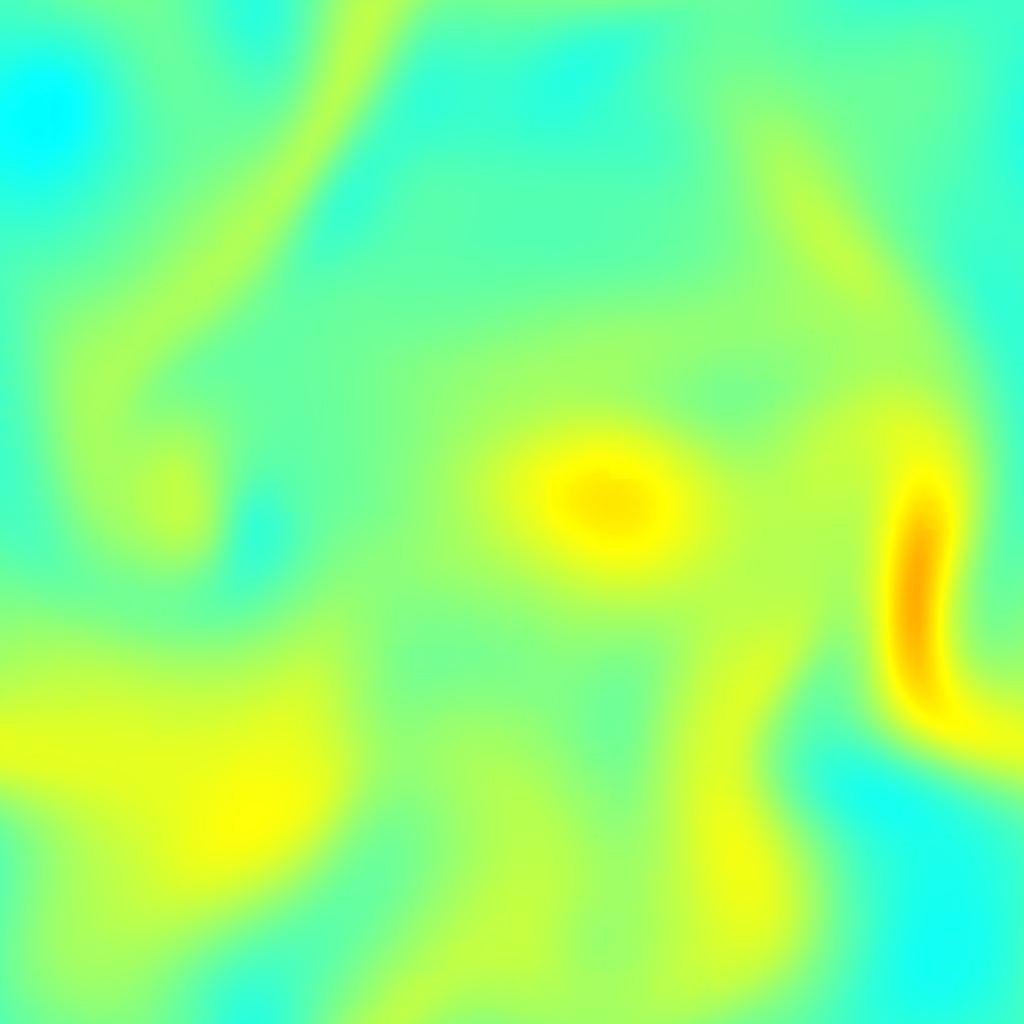
\includegraphics[width=\textwidth,height=0.34\textheight,keepaspectratio]{prec_vitesse_we1.png}\\
      {\scriptsize Vitesse $u_z$}
    \end{column}
    \begin{column}{0.25\textwidth}
      \centering
      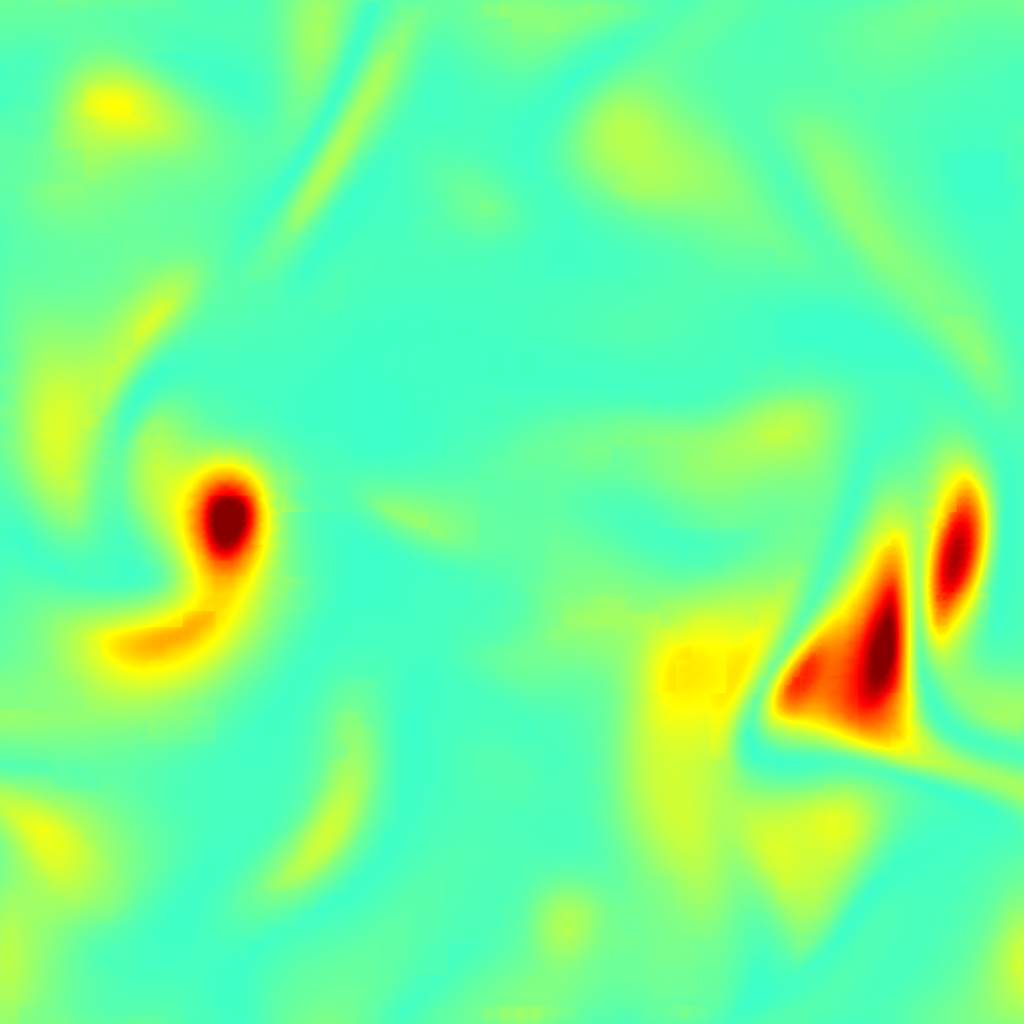
\includegraphics[width=\textwidth,height=0.34\textheight,keepaspectratio]{prec_enstrophie_we1.png}\\
      {\scriptsize Enstrophie $|\boldsymbol\omega|^2$}
    \end{column}
  \end{columns}
  \vspace{0.4em}
  \begin{columns}[c]
    \begin{column}{0.42\textwidth}
      \centering
      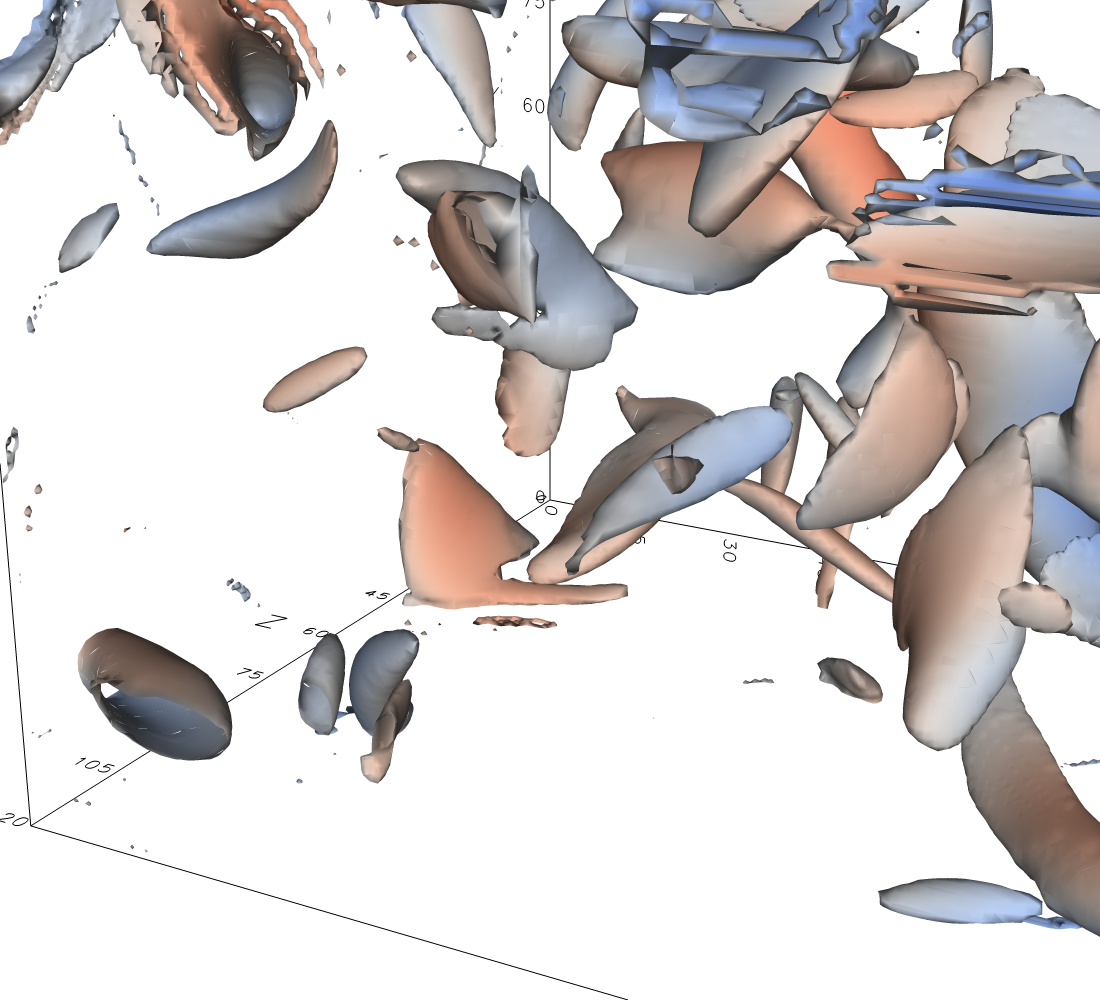
\includegraphics[width=0.78\textwidth,height=0.30\textheight,keepaspectratio]{prec_vortex3d_we1.png}\\
      {\scriptsize Isosurface 3D de $|\boldsymbol\omega|$, colorée par $u_z$.}
    \end{column}
    \begin{column}{0.58\textwidth}
      \footnotesize
      Comparé au champ $KE=200$ : structures tourbillonnaires
      \textbf{plus grosses et moins nombreuses}, maillage nettement plus
      grossier là où l'écoulement est calme --- même physique THI,
      intensité choisie, coût réduit.
    \end{column}
  \end{columns}
\end{frame}

%==============================================================================
\section{Résultats : bulles à $We_t \approx 1$}
%==============================================================================
\begin{frame}{La bulle \emph{survit} : volume conservé, pas de fragmentation}
  \begin{columns}[c]
    \begin{column}{0.62\textwidth}
      \centering
      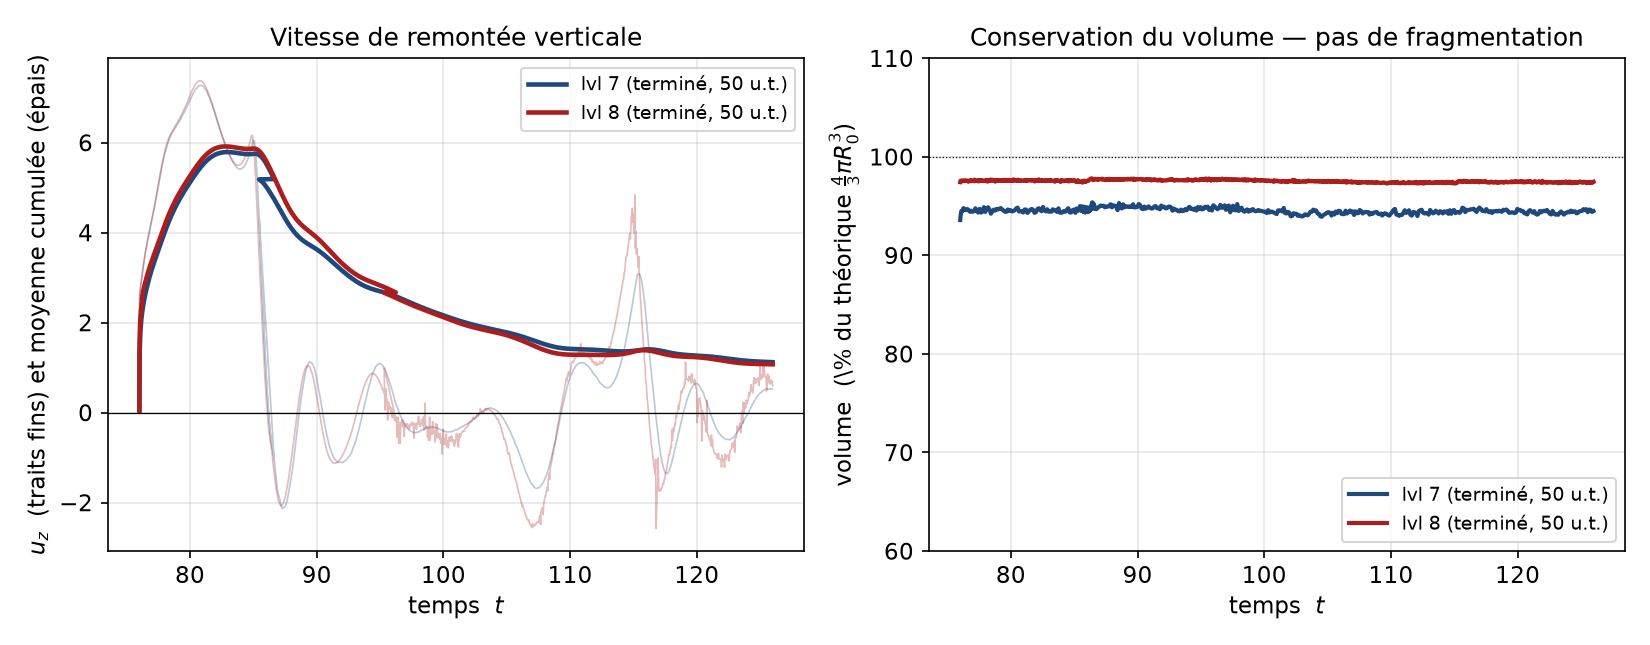
\includegraphics[width=\textwidth]{bulle_we1_uz_volume.png}
    \end{column}
    \begin{column}{0.38\textwidth}
      \footnotesize
      Bulles injectées dans le champ mûr à $t=76$, $R_0=8$, forçage tenu à
      $KE=15$ pendant la remontée.
      \begin{itemize}
        \item \textbf{lvl 7} ($8$ cœurs) : \textbf{terminé}, $50$ u.t. suivies.
        \item \textbf{lvl 8} ($32$ cœurs) : \textbf{terminé aussi}, $50$ u.t.
              (tolérance solveur relâchée à $0{,}1$ pour accélérer).
      \end{itemize}
      \begin{block}{Le point clé}
        \footnotesize
        Volume $\approx \mathbf{94\,\%}$ (lvl 7) et $\mathbf{97\,\%}$ (lvl 8)
        du théorique, \textbf{stable tout du long}. Bulle \textbf{intacte},
        $\chi \lesssim 2{,}5$.
      \end{block}
      \textcolor{okgreen}{\textbf{Contraste net}} avec $We_t=11$ (perte de
      $88\,\%$ du volume, cascade de rupture). Le régime $We_t \approx 1$ est
      bien celui où la vitesse terminale a un sens.
      \vspace{0.2em}
      {\scriptsize\itshape Films (bulle + maillage, vitesse, vorticité) rendus
      aux deux niveaux : \texttt{films/we1\_lvl\{7,8\}\_*.mp4}.}
    \end{column}
  \end{columns}
\end{frame}

\begin{frame}{Vitesse de remontée : \textbf{lvl 7 $\approx$ lvl 8} (convergence)}
  \begin{columns}[c]
    \begin{column}{0.62\textwidth}
      \centering
      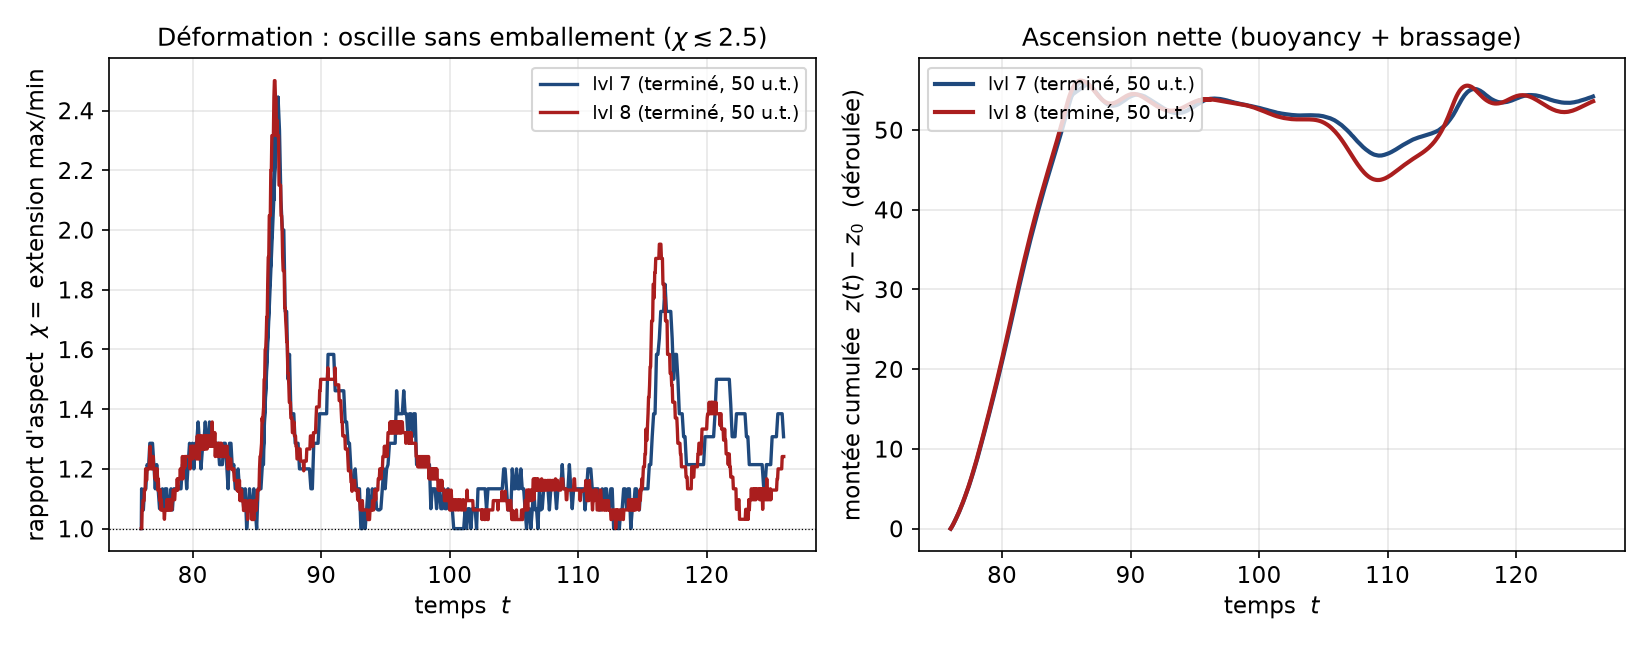
\includegraphics[width=\textwidth]{bulle_we1_aspect_traj.png}
    \end{column}
    \begin{column}{0.38\textwidth}
      \footnotesize
      $u_z$ instantané oscille fortement (la bulle est \emph{brassée} par les
      tourbillons, écart-type $\approx 2{,}5$--$3$) : la remontée se lit sur la
      \textbf{moyenne cumulée} et le déplacement net.
      \begin{block}{Convergence spatiale démontrée (fenêtre complète)}
        \footnotesize
        Déplacement net sur les $\mathbf{50}$ u.t. :
        \[ U_b^{\text{lvl7}} = 1{,}08 \;\approx\; U_b^{\text{lvl8}} = 1{,}07 \]
        ($\approx 1\,\%$) --- et déjà $2{,}79 \approx 2{,}82$ sur les $19$
        premières. Vitesse de remontée \textbf{indépendante du maillage}.
      \end{block}
      La montée est \emph{front-loaded} : rapide au début, puis la bulle
      \textbf{stationne} (montée nette $\approx 0$ sur les $25$ dernières u.t.,
      le brassage domine). $C_D \approx 18$ (effectif, convergé) ; une vitesse
      terminale « propre » demanderait une moyenne d'ensemble.
    \end{column}
  \end{columns}
\end{frame}

\begin{frame}{Récapitulatif chiffré --- $We_t \approx 1$}
  \footnotesize
  \begin{columns}[T]
    \begin{column}{0.58\textwidth}
      \begin{tabular}{@{}lcc@{}}
        \toprule
        \textbf{Grandeur} & \textbf{lvl 7} & \textbf{lvl 8} \\
        \midrule
        Fenêtre suivie (u.t.)                 & $50$ & $50$ \\
        Cellules (adaptatif)                  & $\approx 0{,}66$~M & $\approx 1{,}2$~M \\
        Volume / théorique                    & $94\,\%$ & $97\,\%$ \\
        $\chi$ moyen (max)                    & $1{,}26$ ($2{,}44$) & $1{,}24$ ($2{,}50$) \\
        Fragmentation                         & \textcolor{okgreen}{\textbf{non}} & \textcolor{okgreen}{\textbf{non}} \\ \midrule
        $U_b$ sur $19$ u.t.                    & $2{,}79$ & $2{,}82$ \\
        \rowcolor{okgreen!15}
        $U_b$ net sur $50$ u.t.               & $\mathbf{1{,}08}$ & $\mathbf{1{,}07}$ \\
        $C_D$ effectif ($Re_b \approx 9$)     & $\approx 18$ & $\approx 18$ \\
        \bottomrule
      \end{tabular}
      \vspace{0.4em}\\
      {\scriptsize $\nu \approx 1{,}82$, $D = d_{eq} \approx 15{,}8$ (code).}
    \end{column}
    \begin{column}{0.42\textwidth}
      \begin{block}{Acquis}
        \footnotesize
        \begin{itemize}
          \item Régime $We_t \approx 1$ \textbf{tractable} : bulle intacte,
                solveur sain aux deux niveaux.
          \item \textbf{Convergence maillage} de $U_b$ (lvl 7 $\equiv$ lvl 8).
        \end{itemize}
      \end{block}
      \begin{block}{Prochaine étape}
        \footnotesize
        Prolonger lvl 8 pour une \textbf{vitesse terminale} et un $C_D$
        stationnaires (fenêtre $> 40$ u.t.), puis \textbf{balayer $We_t$}
        de $\sim 0{,}5$ à $\sim 11$ à maillage convergé --- l'étude centrale,
        borne haute $We_t=11$ déjà en main.
      \end{block}
    \end{column}
  \end{columns}
\end{frame}

\begin{frame}{La bulle perturbe-t-elle la turbulence ? \textbf{Presque pas}}
  \begin{columns}[c]
    \begin{column}{0.62\textwidth}
      \centering
      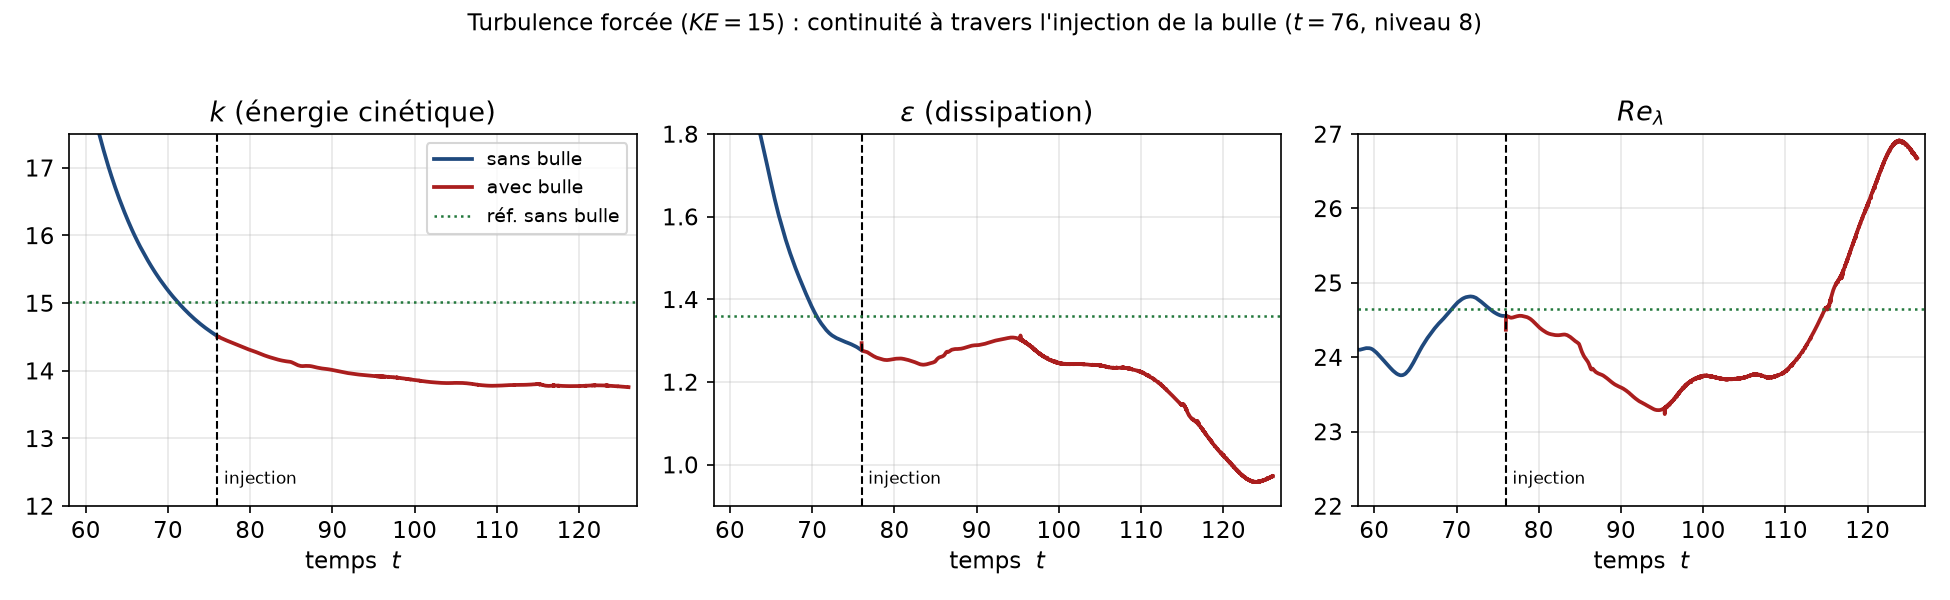
\includegraphics[width=\textwidth]{turbu_avec_bulle.png}
    \end{column}
    \begin{column}{0.38\textwidth}
      \footnotesize
      On compare les grandeurs turbulentes \textbf{avant} (champ ré-équilibré,
      \emph{sans} bulle) et \textbf{après} l'injection ($t=76$), \emph{au même
      niveau 8}. Les courbes sont \textbf{continues} à travers l'injection.
      \begin{center}
      \scriptsize
      \begin{tabular}{@{}lccc@{}}
        \toprule
         & sans & avec & écart \\ \midrule
        $k$        & $15{,}0$ & $13{,}8$ & $-8\,\%$ \\
        $\varepsilon$ & $1{,}36$ & $1{,}18$ & $-13\,\%$ \\
        $Re_\lambda$  & $24{,}6$ & $24{,}4$ & $-1\,\%$ \\
        $\eta$        & $1{,}45$ & $1{,}51$ & $+4\,\%$ \\
        \bottomrule
      \end{tabular}
      \end{center}
      \begin{block}{Interprétation}
        \footnotesize
        Une seule bulle occupe $\sim 0{,}1\,\%$ du volume : les stats globales
        restent à $\lesssim 10\,\%$ du champ initial, sans saut à l'injection
        $\Rightarrow$ \textbf{couplage essentiellement à sens unique} (une part
        de la dérive tardive est l'évolution propre du champ, pas la bulle). La
        turbulence caractérisée reste \emph{représentative}.
      \end{block}
    \end{column}
  \end{columns}
\end{frame}

%==============================================================================
\section{Synthèse}
%==============================================================================
\begin{frame}{Synthèse de la semaine}
  \begin{columns}[T]
    \begin{column}{0.5\textwidth}
      \textbf{Acquis}
      \begin{itemize}
        \item Précurseur THI mûr, \textbf{caractérisé quantitativement}
              ($Re_\lambda \approx 45$, toutes échelles résolues,
              preuves aux niveaux 7/8/9).
        \item AMR-vorticité validée : contourne la limite machine
              \emph{et} économise $\times 2{,}5$ en mailles.
        \item Premier run bulle complet + post-traitement entier
              (trajectoire, $u_z$, $\chi$, volume).
        \item Recette de ré-équilibrage : l'intensité turbulente est
              maintenant un \textbf{bouton réglable} (peu coûteux).
      \end{itemize}
    \end{column}
    \begin{column}{0.5\textwidth}
      \textbf{Enseignement principal}
      \begin{alertblock}{$We_t$ pilote tout}
        \footnotesize
        À $We_t \approx 11$, la bulle $Bo=1$ \textbf{fragmente} : pas de
        vitesse terminale mesurable. À $We_t \approx 1$, elle reste
        \textbf{intacte} aux deux niveaux et $U_b$ est \textbf{convergé}
        (lvl 7 $\equiv$ lvl 8, $1\,\%$) --- la mesure vitesse/traînée
        devient possible.
      \end{alertblock}
      \textbf{Points ouverts}
      \begin{itemize}
        \item Vitesse terminale « propre » / $C_D$ : la montée nette est
              \emph{front-loaded} (nulle sur les $25$ dernières u.t.)
              $\Rightarrow$ moyenne d'ensemble ou run plus long.
        \item lvl 9 : nécessite de plafonner l'AMR vorticité au niveau 8
              (différé).
        \item Balayage en $We_t$ ($0{,}5 \to 11$) à maillage convergé.
      \end{itemize}
    \end{column}
  \end{columns}
\end{frame}

{\setbeamertemplate{footline}{}
\begin{frame}[plain]
  \centering
  \vfill
  {\Large\bfseries\color{imftblue} Merci de votre attention}\\[0.4cm]
  {\normalsize Questions \& discussion}\\[0.8cm]
  
\includegraphics[height=1.0cm]{logo_enseeiht.png}\hspace{1.2cm}
  
\includegraphics[height=1.0cm]{logo_imft.png}
  \vfill
\end{frame}}

\end{document}
